\chapter{Theme 1: Modeling the Physiological Environment}

Closed-loop medical devices such as the implantable cardiac pacemaker and defibrillator are designed to operate autonomously and interact with the human body to maintain and improve the physiological conditions of the patients. To evaluate the device within the closed-loop context of the human body, the knowledge of the physiological contexts (e.g. patient arrhythmia, physical activity) and the signals by which the device interacts with the organ(s) to manage the condition is essential. By constructing physiological models and encoding physiological requirements, our goal is to evaluate the safety and efficacy of the device therapy across a range of physiological conditions. 

Consequently, it is important to model the physiological environment of the device such that details unrelated to the interaction between the device and the human are abstracted away, while essential information required to differentiate different patient conditions are maintained. As we will see, to validate the device operation across a range of physiological conditions and for a set of safety and efficacy properties, a family of models are needed which refine the closed-loop context to appropriately express the condition to be verified.

%\newpage
%\begin{itemize}
%\vspace{-5pt}
%\item How does the device interact with the physiological environment?
%\vspace{-5pt}
%\item What details must the physiological environment models capture?
%\vspace{-5pt}
%\item What are the different modeling philosophies when developing environment models for testing and for model checking?
%\end{itemize}

Models, especially models of the human physiology, which span a large spectrum of scale and complexity, should be designed in accordance with their respective applications. Each application of the environment model has a different focus and has distinct modeling requirements which influence the model complexity and model identifiability.

\textbf{Model complexity:} How much detail should the physiological models have, in order to unambiguously describe a physiological behavior? In particular, if the model checker returns an execution trace as counter-example, how much details should the physiological model have so that the execution traces can be interpreted by domain experts? 	

\textbf{Model Identifiability} is a metric for the feasibility of identifying model parameters from data. There are two methods for model construction: non-parametric modeling in which no prior knowledge is assumed and the model construction is purely data-driven; and parametric modeling in which domain knowledge of the physiological conditions is taken into account. For example, to model the electrophysiological activity of the heart, there is abundant literature describing the phenomena of individual arrhythmia, which makes parametric modeling of the environment favorable.

%%It affects the validity of the model which is a key element for closed-loop verification. Model identifiability is generally affected by the model complexity and the availability and quality of clinical data. 

%%The complexity requirements of an environment model is usually determined by 1) The complexity of the interactions between the environment model and the system model and 2) The complexity of the environment condition specified in the physiological requirements.

In the following sections, we introduce the physiological contexts within which the implantable pacemaker operates, and proceed to construct a heart model structure for closed-loop validation of the pacemaker. Note that for two different applications, i.e. model checking of the device model in the loop and functional testing of the actual device in the loop, models are constructed differently as we address their respective requirements for environment models. 



\begin{figure}[!t]
\centering
		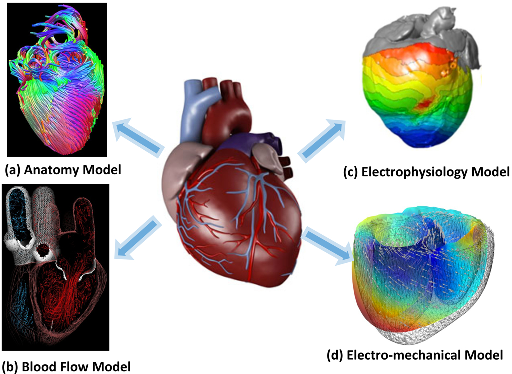
\includegraphics[width=0.9\textwidth]{figs/models.pdf}
		
%\vspace{-10pt}
\caption{\small Physiological models of the heart from different perspectives}
\label{fig:models}
%\vspace{-15pt}
\end{figure} 
\section{Physiological Models of the Heart}
To study the mechanisms of heart diseases and their effects on cardiac output, different physiological models of the heart have been developed. \figref{models} illustrates several aspects that these models capture. With the development of the imaging techniques like MRI, detailed anatomical structures of the heart can be modeled and studied (\cite{geometric}). These models are fundamental in other modeling aspects as well, as the anatomy of the heart dictates the electrical and mechanical behaviors of the heart. \figref{models}.(a) shows models for heart muscle fiber orientations by \cite{fiber}. With anatomy models the electrical and/ or mechanical properties of the heart can be studied. \figref{models}.(b) illustrate a model of blood flow within the ventricles (\cite{bloodflow}). Electrical properties of the heart at cellular level has been modeled (\cite{cellular}) and by combining these cellular models with the structural models, the electrical activities of the whole heart are studied, especially the mechanism of different arrhythmia (\cite{natalia},~\cite{Grosu_MHA},~\cite{Grosu_wave}). Intrinsic heart rate variability has been modeled to synthesize optimal control of pacemaker pacing. (\cite{Bogdan}) Abstraction of the electrical cellular model has also been attempted by \cite{Grosu_abstract} to reduce model complexity without sacrificing accuracy. The electrical properties and the mechanical properties of the heart are closely coupled. Models combining both of these aspects are also developed to study the effects of different arrhythmia on cardiac outputs (\cite{natalia},~\cite{eletro_mechanical}).

\section{EP Heart Model Structure for Closed-loop Validation of Implant-able Cardiac Devices}
Models should be developed according to their applications. The aforementioned models of the heart are mostly used for understanding the mechanisms of different heart diseases. Physiological models developed for closed-loop evaluation of medical devices should have the following considerations:\\
\textbf{C1. Interfacing with the device: }The model should be able to generate physiological signals that the device sense from the real physiological entities. And the model should be able to take device output as input and change its states accordingly. Model complexity should also be adjusted according to the device interface to hide unnecessary details.\\
\textbf{C2. Differentiate different physiological conditions: }To evaluate the safety and effectiveness of the device, the device has to be evaluated under certain physiological conditions specified by the requirements. For example, the pacemaker is supposed to maintain proper heart rate during Bradycardia. The model should be expressive enough to be able to differentiate the physiological condition (Bradycardia in the example) from other conditions. Failing to do so may result in false-positives or false-negatives in the evaluation result. \\
\textbf{C3. Physiological/logical interpretation of model states: } In closed-loop evaluation we are checking the device safety and effectiveness against the physiological requirements. However, due to the limited interface (e..g two leads for a dual chamber pacemaker) it is always difficult to determine only from an execution trace that the therapy is safe and effective. Therefore, being able to provide physiological meanings to the states of the model also allows us to interpret the closed-loop execution more accurately, thus reducing the number of physiologically impossible executions during the evaluation. To satisfy these requirements, the model structure of these physiological models should base on physiological or clinical first principles so that states and state transitions of the closed-loop executions can be explained with physiological language. \\%One advantage of closed-loop evaluation over open-loop evaluation is the capability to provide physiological/logical interpretation of an execution trace. With this advantage we are able to identify and reduce the number of physiological-impossible executions by examining the state of the model, so that the evaluation can focus on physiological-possible executions. This requires the model first-principle\\
\textbf{C4. Available patient data: } In closed-loop evaluation, physiological models are developed to represent certain physiological condition across a population of patients or even a particular patient. The model parameters must be identified so that the behaviors of the models match the behaviors of the patients (groups).  Due to the limited sensing capability of closed-loop medical devices, the obtained data is sparse. i.e. we can not put a sensor on every tissue region of the heart. Therefore the complexity of the model should be in accordance with the available data to avoid \emph{over-fitting}, which occurs when a model has too many parameters relative to the number of observations, and this can introduce errors during prediction. 

The electrophysiological models mentioned in the last section (\cite{natalia,Grosu_MHA}) satisfy C1-C3. However, the parameter space of these models are too large (10+ parameters for each cellular model multiplied by $10^5$ of elements) which not only increase simulation complexity, but also impossible to identify due to lack of data. As introduced in Section \ref{EP}, the pacemaker has only two leads at fixed locations and only use timing between local activation events for diagnosis. These models with high spatial fidelity possess details that can be abstracted without sacrificing the three considerations.

Electrophysiology testing (EP testing) has been an active clinical field to diagnose and treat arrhythmia with minimal-invasive procedures. During an EP testing procedure, the physicians diagnose heart conditions by examining the patterns and intervals of local electrical activations (temporal) measured from electrodes placed into different locations of the heart (spatial). EP testing is the perfect modeling level for closed-loop evaluation of implantable cardiac devices because: 1) it is the basis of implantable cardiac devices (C1), 2) physicians can use EP testing to diagnose most arrhythmia thus distinguish them (C2,C3), 3) there are abundant patient data available (C4). 

In the remaining chapter we will introduce our heart modeling efforts based on EP testing, and model adaptation for two different applications of closed-loop evaluation of implantable cardiac devices.
%\section{Heart Models for Pacemaker Interaction}
%The heart generates electrical impulses to maintain the heart rate appropriate for the physiological needs. These impulses conduct through the heart, triggering coordinated muscle contractions which pumps blood to the rest of the body. The underlying pattern and timing of these impulses determines the heart's rhythm and is key to proper heart function. Derangements in this rhythm are referred to as \emph{arrhythmia}, which 



%\subsection{Electrical conduction system of the heart}
%Heart tissue with different timing parameters form the electrical conduction system to ensure coordinated contraction of the heart. First, specialized tissue at the Sinoatrial (SA) node periodically and spontaneously self-depolarizes. This is controlled by the nervous system and the SA node is the primary and natural pacemaker of the heart. The activation signal then travels through both atria, causing contraction and pushes blood into the ventricles. Then the activation is delayed at the Atrioventricular (AV) node which allows the ventricles to fill fully. The fast-conducting His-Purkinje system then spreads the activation signal within both the ventricles. The simultaneous contraction of the ventricle muscles will push the blood out of the heart.
%\begin{figure*}[!t]
%\centering
		%\subfigure [\small]{			
		%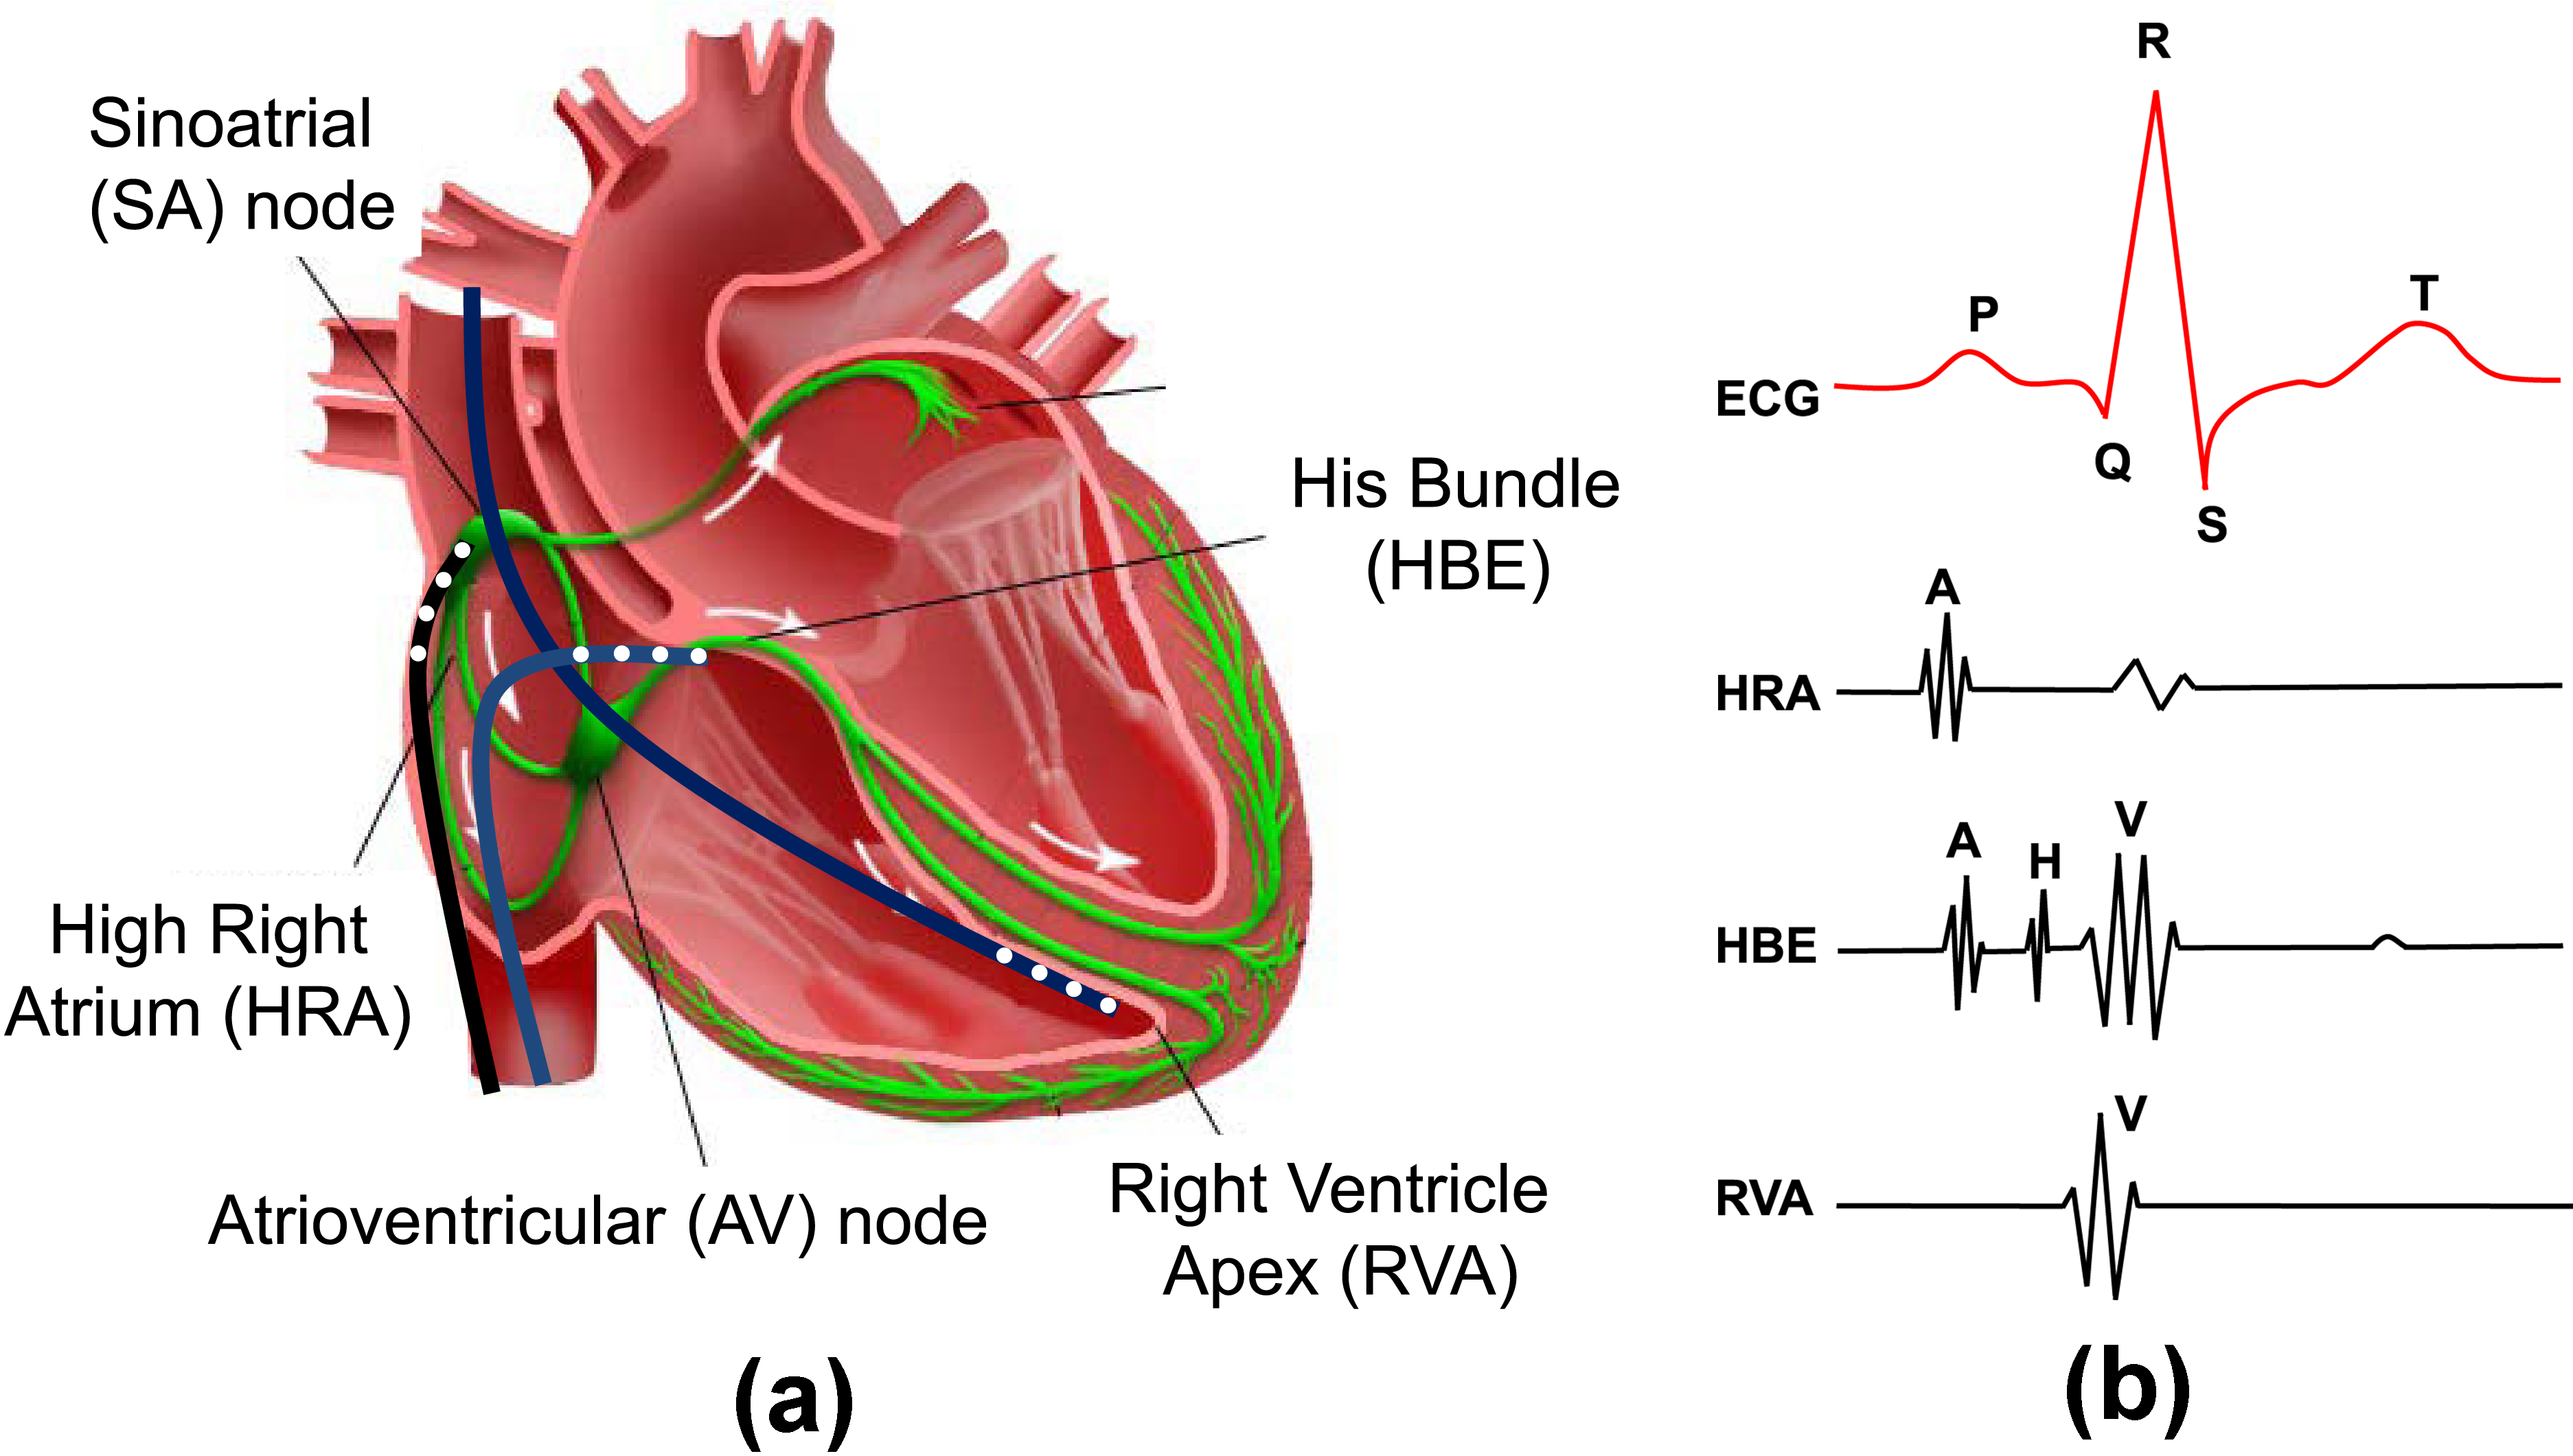
\includegraphics[width=0.3  \textwidth]{figs/probes.png}
		%\label{fig:probes}
		%} 
%
		%\subfigure [\small] 
		%{
		%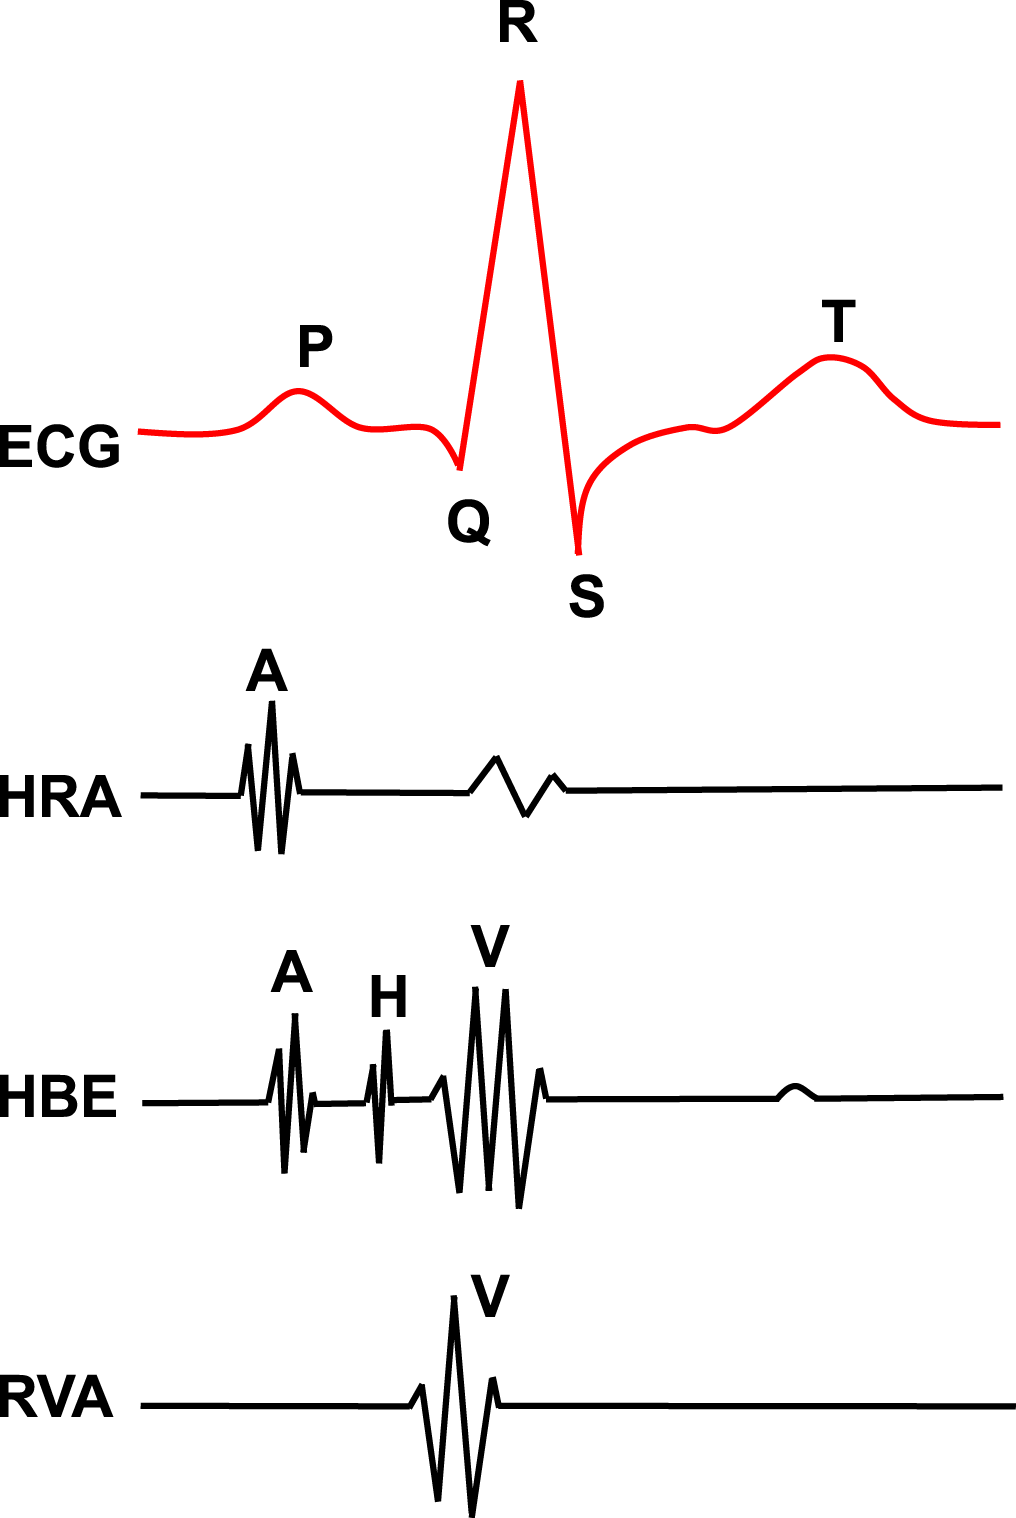
\includegraphics[width=0.2\textwidth]{figs/egm.png}
		%\label{fig:egm}
		%} 
%%\vspace{-10pt}
%\caption{\small (a) Node automaton. Dotted transition is only valid for pacemaker tissue like SA node; (b) Path automaton; (c) Model of the electrical conduction system of the heart using a network of node \& path automata~\cite{vhm_ecrts10}.}
%%\vspace{-15pt}
%\end{figure*} 

%\section{Electrophysiological Testing}
%\Hao{A figure for heart and pacemaker}

%\chapter{Modeling the Physiological Environment}
%\begin{itemize}
	%\item How to encode domain knowledge of the physiological environment into models?
    %\item What are the applications that the models will be used?
    %\item What are the differences in terms of environment models between model checking and simulation?
    %\item How to balance complexity and expressiveness of the model?
%\end{itemize}

%In the following sections, we demonstrate how to construct heart models for closed-loop verification of implantable pacemaker. Note that for two different applications the models are constructed differently as we address their respective requirements for environment models. 


%\begin{itemize}
	%\item Why the models at this level have to be deterministic? Where can they be used?
    %\item How electrophysiology reflects the functions of the heart?
    %\item How to encode these knowledge into models?
    %\item Why VHM has the right level of details for pacemaker verification?
    %\item How VHM interacts with pacemaker?
    %
%\end{itemize}
%During closed-loop testing, the devices interact with the environment (or its models) under different environmental conditions. The closed-loop executions are monitored and violations of safety and efficacy requirements are reported. In model-based closed-loop testing, the environment models are expected to mimic the behaviors of actual environment and its interaction with the device. Thus, the environment models are in general deterministic so that the execution traces are reproducible and are able to mimic different arrhythmia. Complex dynamics during state transitions also need to be captured to validate violations within longer executions traces. 

\subsection{Modeling Philosophy}
As the pacemaker can only sense and actuate from two locations within the heart, only structures and parameters that affect inputs to the pacemaker are needed. Since the two leads are fixed, the accurate spatial locations of different heart anatomical structures are not necessary. Instead, the topology of the electrical conduction system of the heart is more important. 


\begin{figure}[!t]
\center
%\vspace{-10pt}
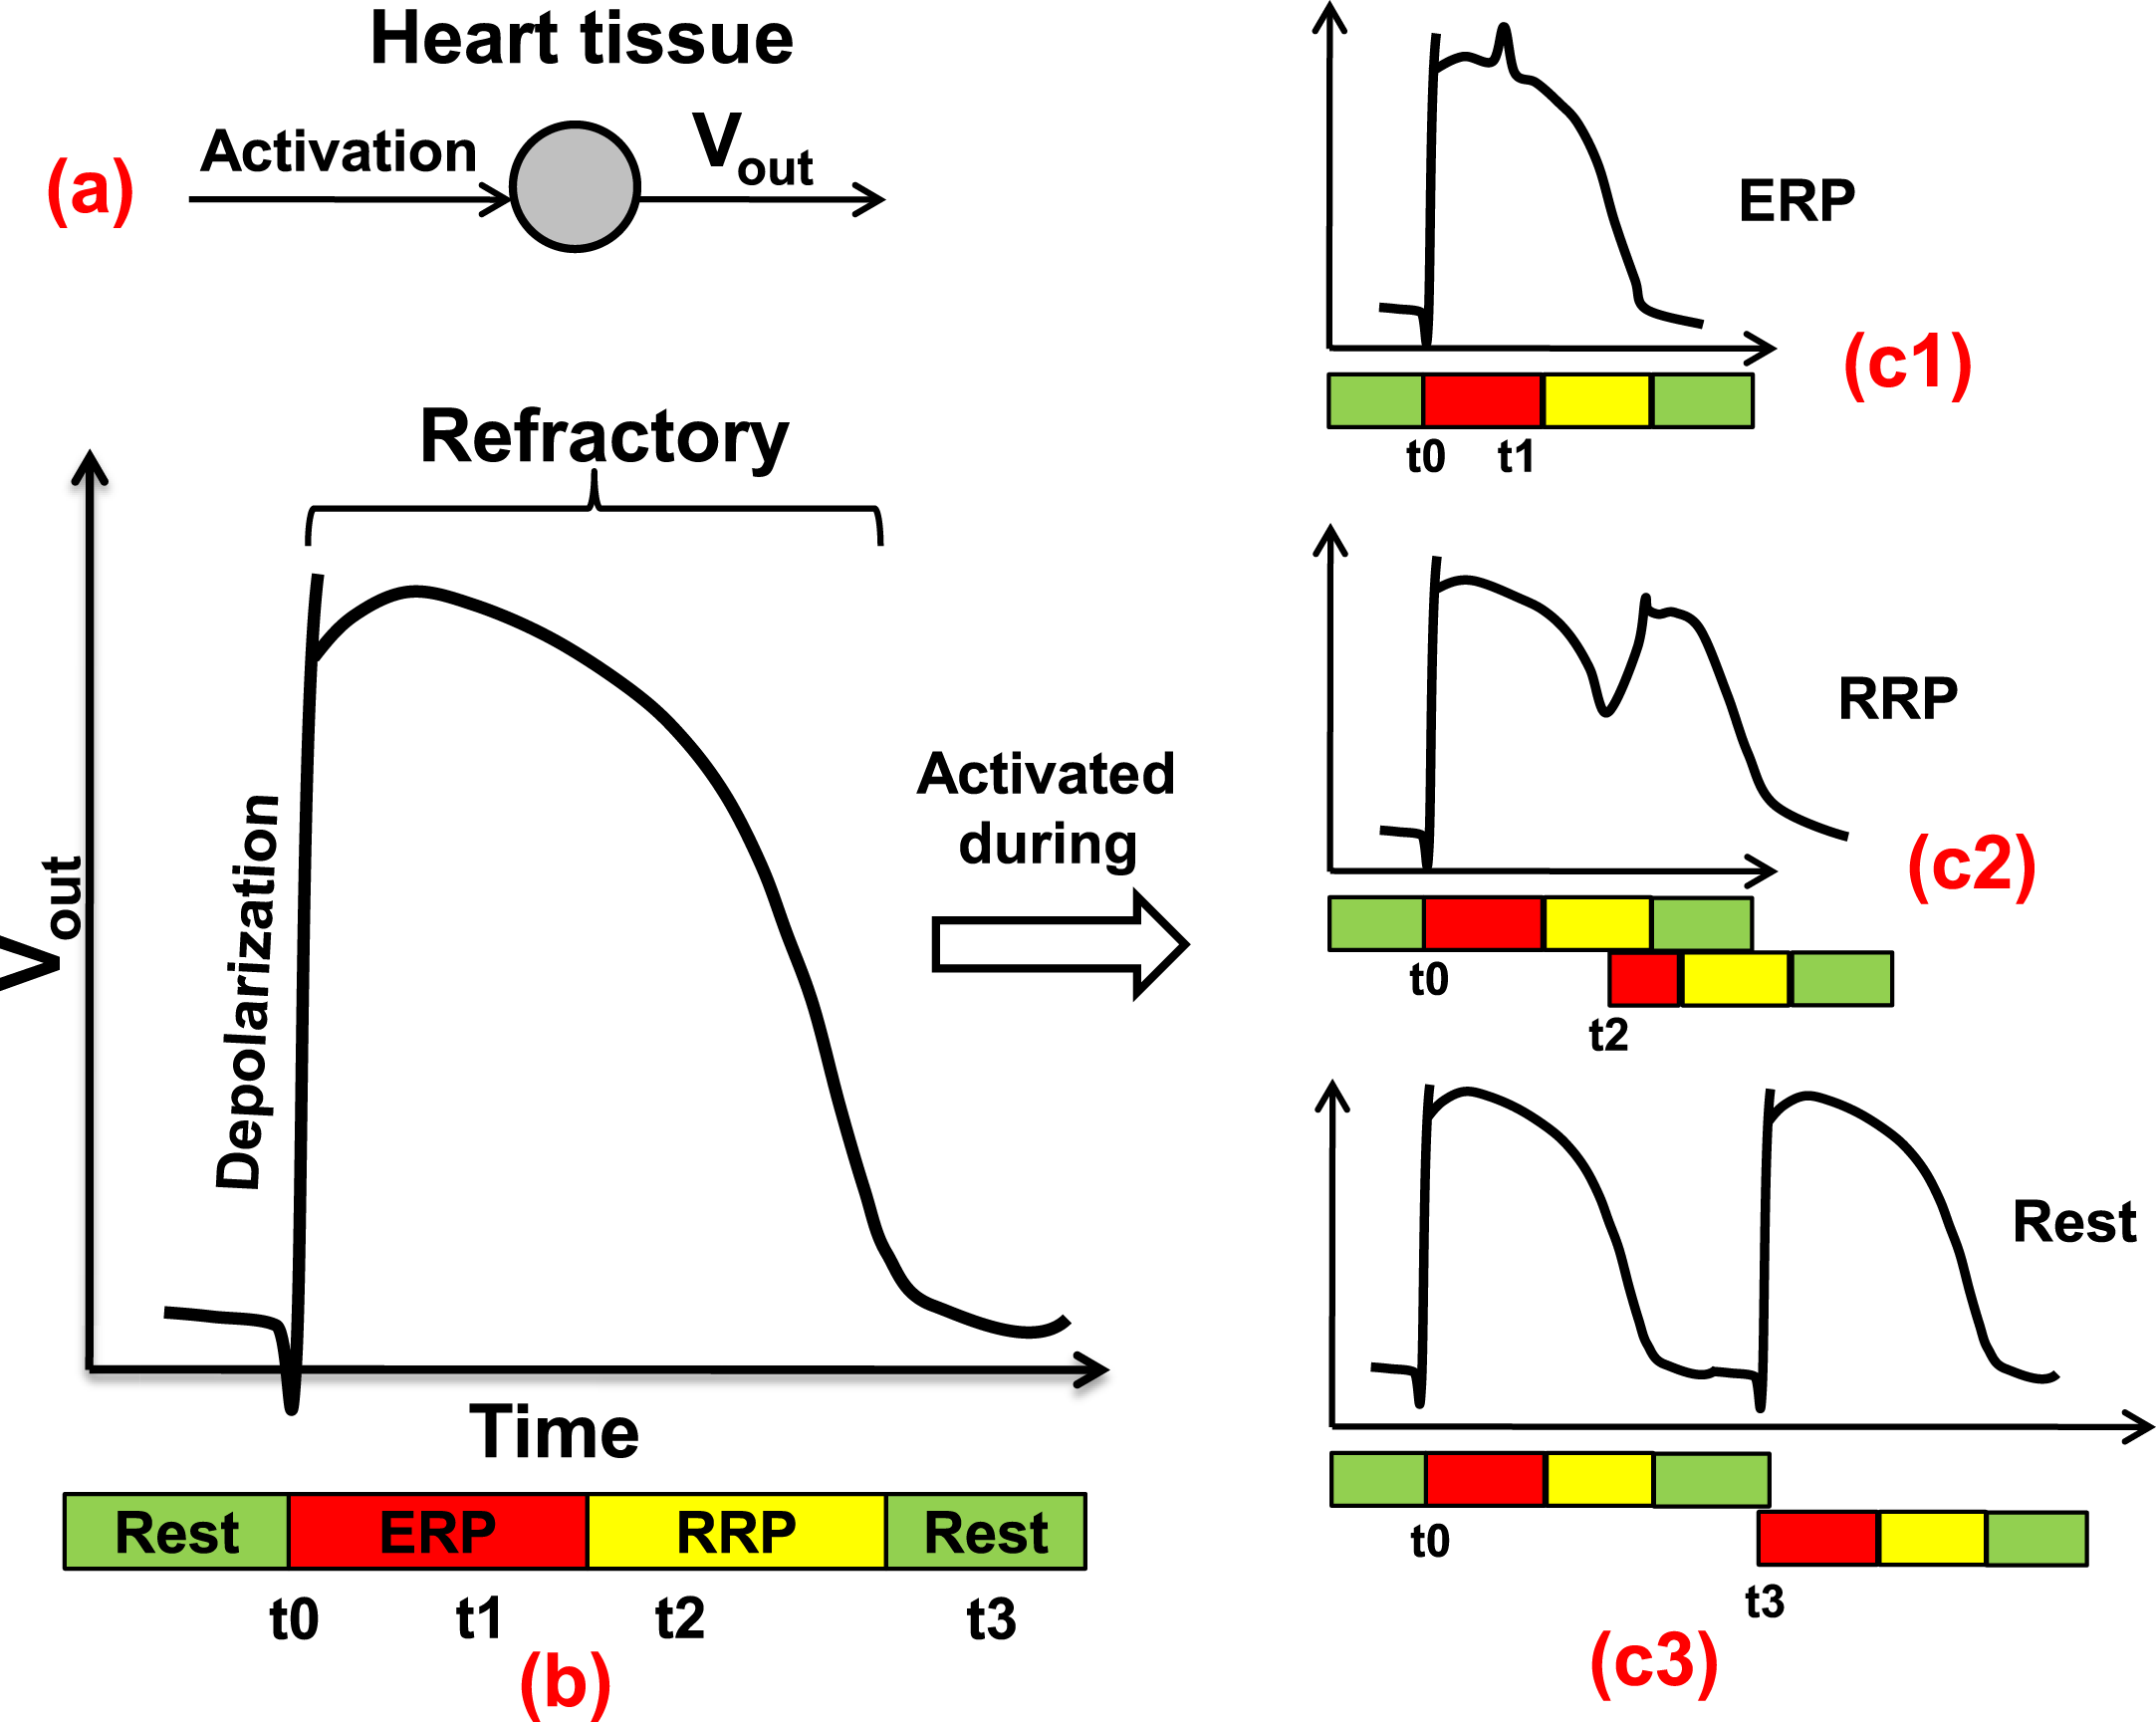
\includegraphics[width=0.7\textwidth]{figs/refractory.png}
%\vspace{-10pt}
\caption{(a) The generation of Action potential; (b) Action potential; (c1) The second activation arrived during ERP; (c2) Arrived during RRP; (c3) Arrived after refractory.}
\label{fig:refractory}
%\vspace{-10pt}
\end{figure} 
\subsection{Timing Behaviors of Cellular Electrophysiology}
The contraction of heart muscles is triggered by external voltage applied to the tissue. After the activation, a transmembrane voltage change over time can be sensed due to ion channel activities, which is referred to as an Action Potential (\figref{refractory}(a)). The upstroke of the action potential is called depolarization, during which the muscle will contract. The voltage change caused by the depolarization will depolarize the tissue nearby, which causes an activation wave across the heart. After the depolarization there is a refractory period during which the tissue recovers to the pre-excitation state and the voltage drops down to the resting potential. The refractory period can be divided into \emph{Effective Refractory Period (ERP)} and \emph{Relative Refractory Period (RRP)} (\figref{refractory}(b)). During ERP, the tissue cannot be depolarized due to the lack of charge. As a result, the activation wave will be "blocked" at the tissue during ERP (\figref{refractory}(c1)). During RRP, the tissue is partially recovered and the tissue can be depolarized. However, the new action potential generated by the depolarization will have different morphology (e.g. attenuated in magnitude and duration), thus affecting the refractory periods of the tissue and conduction delay of the activation wave (\figref{refractory}(c2)). \figref{refractory}(c1)-(c3) show the action potential shape change and corresponding timing change in refractory periods when the tissue is activated at time stamp $t1$, $t2$, $t3$ after the initial activation $t0$. 

\subsection{Heart Model Components}
We introduce the model components that can be used to configure heart models corresponding to different heart conditions. As discussed earlier, the action potential of a heart tissue has 3 timing periods during which the tissue responds to external electrical stimuli differently. We use an extended timed-automata formulation (\cite{timed_automata}) to model the timing behaviors of a heart tissue during each cycle. 

\textbf{Node Automata:} We refer to the tissue model as \emph{node automaton} and \figref{automata}.(a) shows the structure of a node automaton $i$. 3 states correspond to the timing periods of the action potential. From \textsf{Rest} state, the node can either self-activate or get activated by external stimuli (Act\_node) and go to \textsf{ERP} state. During \textsf{ERP} state the node does not respond to external stimuli (blocked). During \textsf{RRP} state, the node can still be activated and go to \textsf{ERP} state, however the ERP period and the conduction delay of the tissue are affected by the "earliness" of the activation arrived during the RRP period, which is tracked by a shared variable $C(i)$. The new ERP period is determined by a function over clock value $g(f(t))$ which mimics the beat-to-beat dynamics described in \cite{josephson}. The function $g$ and $f$ are given by:
\begin{equation} \label{factor}
						f(t) = 1-t/Trrp
						\end{equation}
and
%  The AV node has a different profile than the other tissue. The ERP period increases rather than decreases when activated during its RRP (~\cite{josephson}).
\begin{equation} \label{earliness_noAV}
						g(x) = \left\{
						\begin{array}{lr}
						
						T_{min}+(1-(1-x)^3)\cdot (T_{max}-T_{min}), i=AV\\
						T_{min}+(1-x^3)\cdot (T_{max}-T_{min}),i\neq AV
			
						
						\end{array}
						\right.
						\end{equation}  
where $T_{min}$ and $T_{max}$ are the minimum and maximum value for \emph{Terp} of the tissue.
\begin{figure}[!t]
%\centering
		%\subfigure [\small]{			
		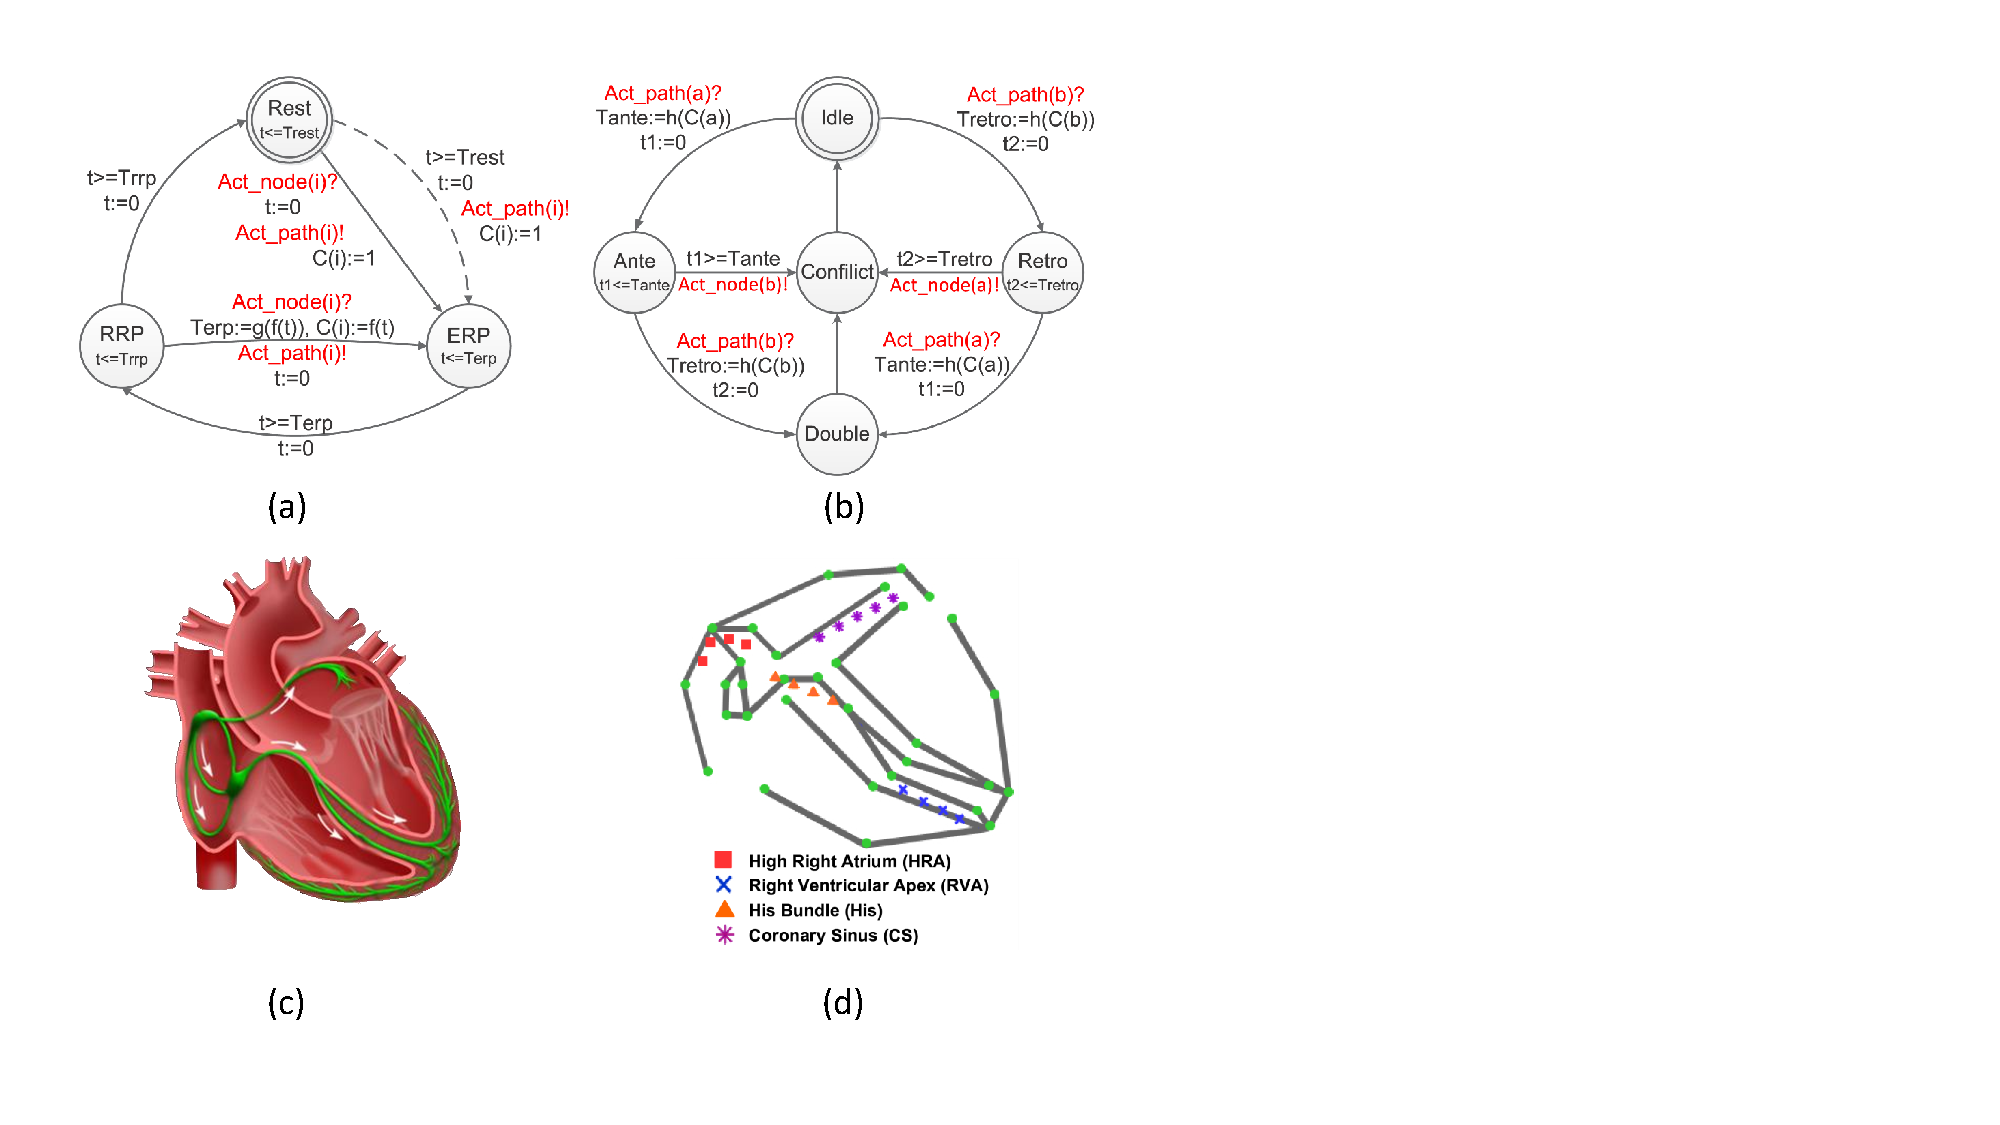
\includegraphics[width=\textwidth]{figs/automata.pdf}
		%\label{fig:node_automata}
		%} 
%%	\hspace{.1in}%
		%\subfigure [\small] 
		%{
		%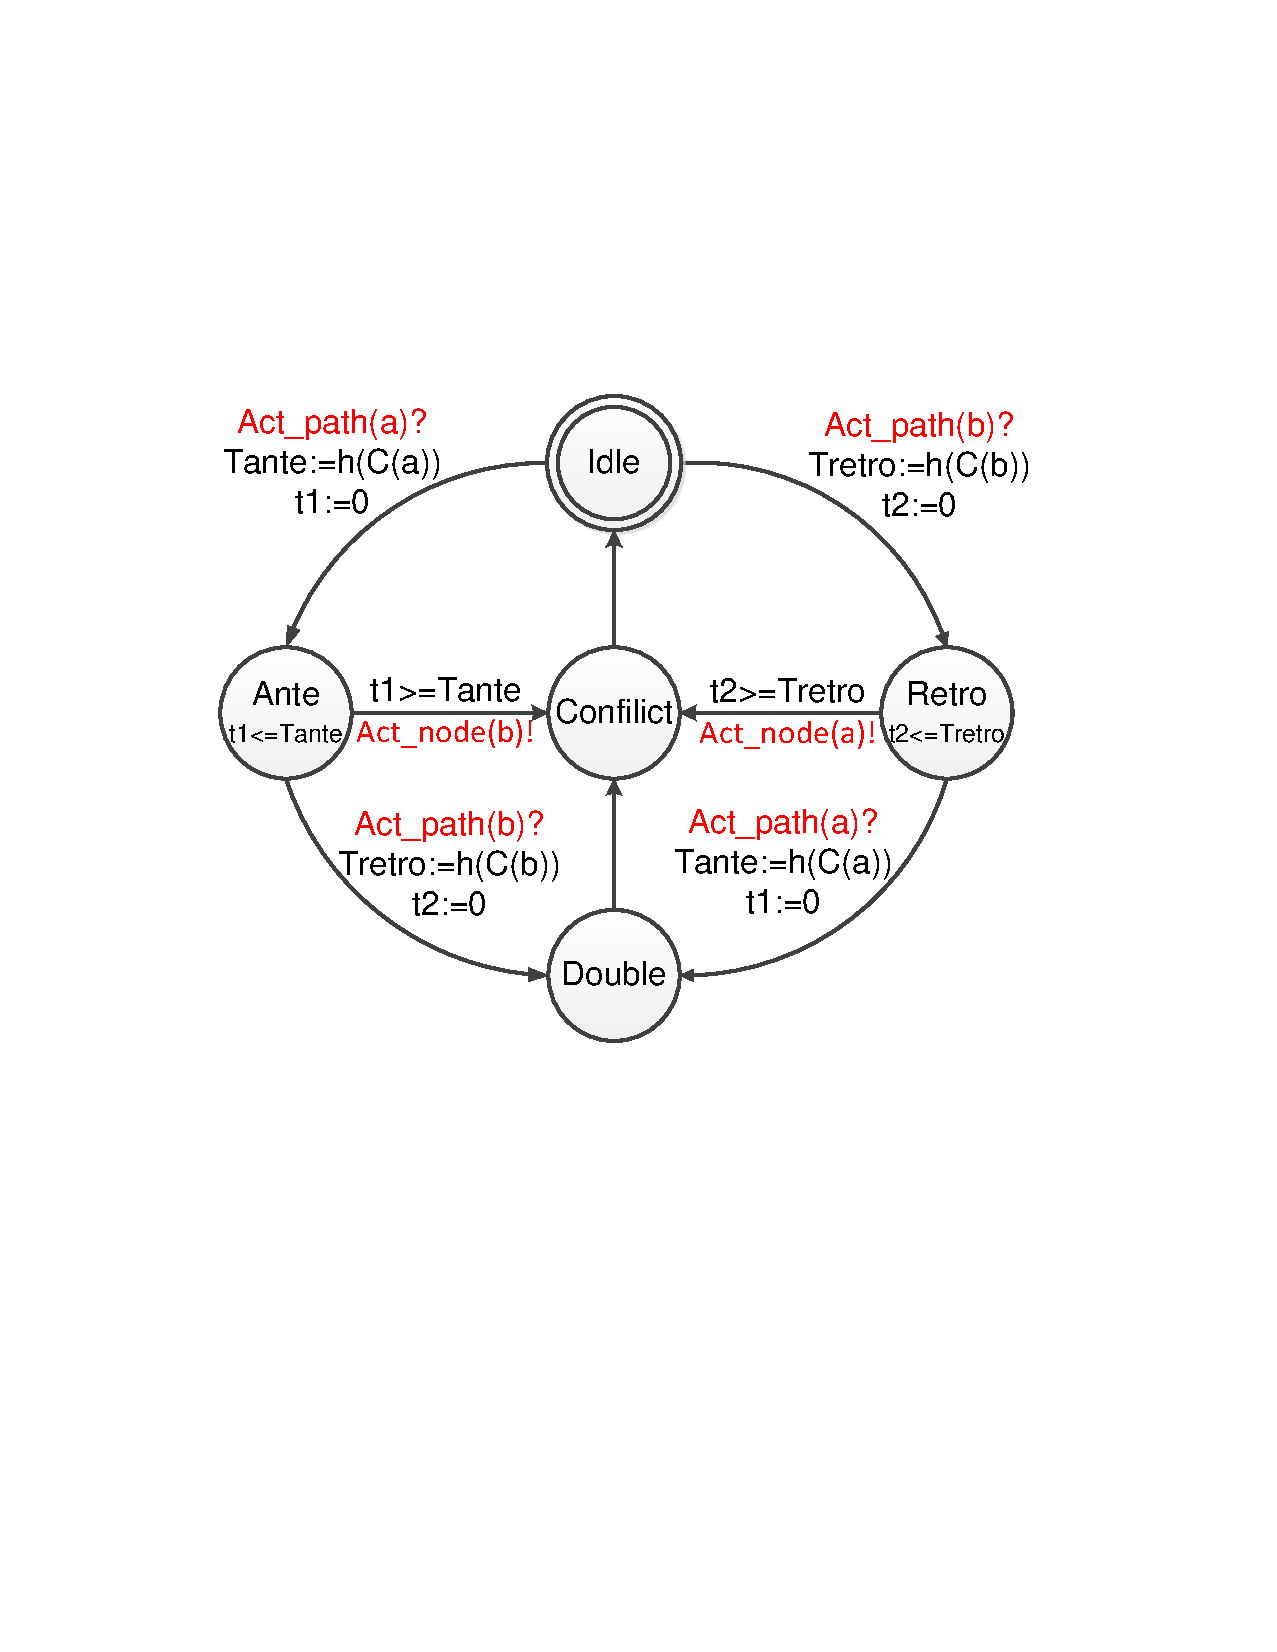
\includegraphics[width=0.32\textwidth]{figs/path.pdf}
		%\label{fig:path_automata}
		%} 
		%\subfigure [\small] 
		%{
		%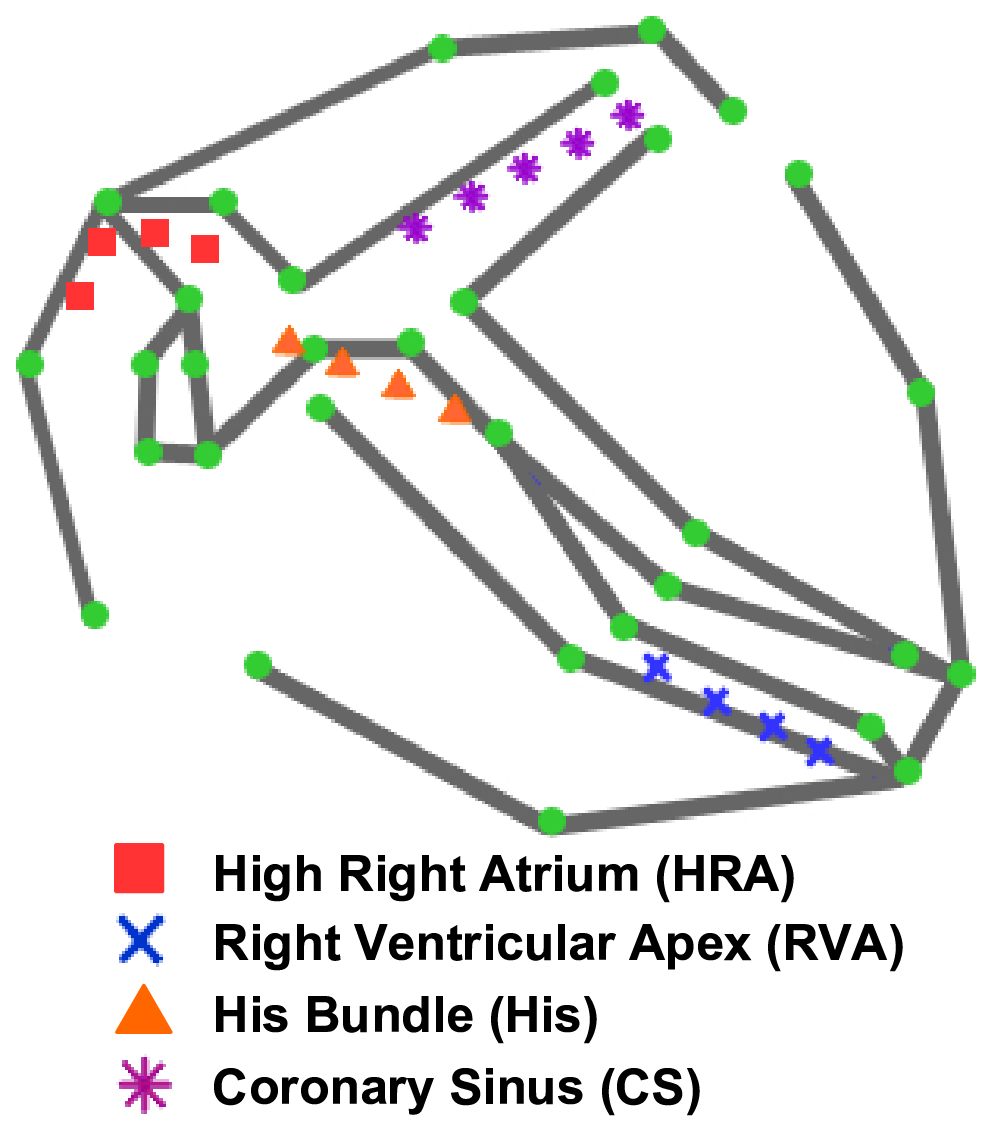
\includegraphics[width=0.25\textwidth]{figs/gen_setup.png}
		%\label{fig:general_setup}
		%} 

%\vspace{-10pt}
\caption{\small (a) Node automaton: The dotted transition is only valid for tissue (like SA node) that can be activated by an external trigger; (b) Path automaton modeling the electric conduction and propagation between two node automata; (c) Electrical conduction system of the heart; (d) Model of the electrical conduction system of the heart using a network of node \& path automata ~\cite{VHM_proc}.}\label{fig:automata}
%\vspace{-15pt}
\end{figure} 

Due to the limited number of observable points within the heart, modeling the electrophysiological behavior of every tissue of the heart and its full anatomy is unnecessary and unfeasible. In our heart models, only self-activating tissue and key hubs of the electrical conduction system are modeled as node automata. 

\textbf{Path Automata:} The electrical conduction through the tissue between nodes are abstracted using \emph{path automata}. The path automata can be used to represent structural or topological (functional) electrical connections between nodes. \figref{automata}.(b) shows a path automaton connecting node a and b.

The initial state of a path automaton is \emph{Idle}, which corresponds to no conduction. The states corresponding to the two conduction directions are named after the physiological terms: Antegrade (Ante) and Retrograde (Retro). These states can be intuitively described as forward and backward conductions. If path actuation \emph{Act\_path} event is received from one of the nodes connected to it, there is a transition to \emph{Ante} or \emph{Retro} state based on the activation source in the path automaton. At the same time, the clock invariant of the state is modified according to the shared variable \emph{C(a/b)}. This corresponds to the change of the conduction delay that is caused by the early activation. Similar to node automaton, the changing trend is extracted from clinical data and the function $h$ is defined as:
\begin{equation} 
						h(c) = \left\{
						\begin{array}{lr}
						
						path\_len/v\cdot (1+3c), i=AV\\
						path\_len/v\cdot (1+3c^2), i\neq AV
						\end{array}
						\right.
						\end{equation}
where $path\_len$ denotes the length of the path and $v$ is the conduction velocity.

After \emph{Tante} or \emph{Tretro} time expires, the path automaton sends out \emph{Act\_node(b)} or \emph{Act\_node(a)} respectively. A transition to \emph{Conflict} state occurs followed by the transition to \emph{Idle} state. The intermediate state \emph{Conflict} is designed to prevent back-flow, where the path is activated by the node \emph{b} it has just activated. If during \emph{Ante} or \emph{Retro} state another \emph{Act\_path} event is received from the other node connected to the path automaton, a transition to \emph{Double} state will occur, corresponding to the two-way conduction. In this case, the activation signals eventually cancel each other and the transition to \emph{Idle} state is taken.

\subsection{Modeling the Heart's Electrical Conduction System}
The node and path automata are the basic building blocks for EP heart modeling. Hearts with different conditions are modeled by using different conduction topologies with appropriate timing parameters for each node and path automata. \figref{automata}.(d) shows one such topology of a network of node and path automata.
\begin{figure}[!t]
\center
%\vspace{-15pt}
		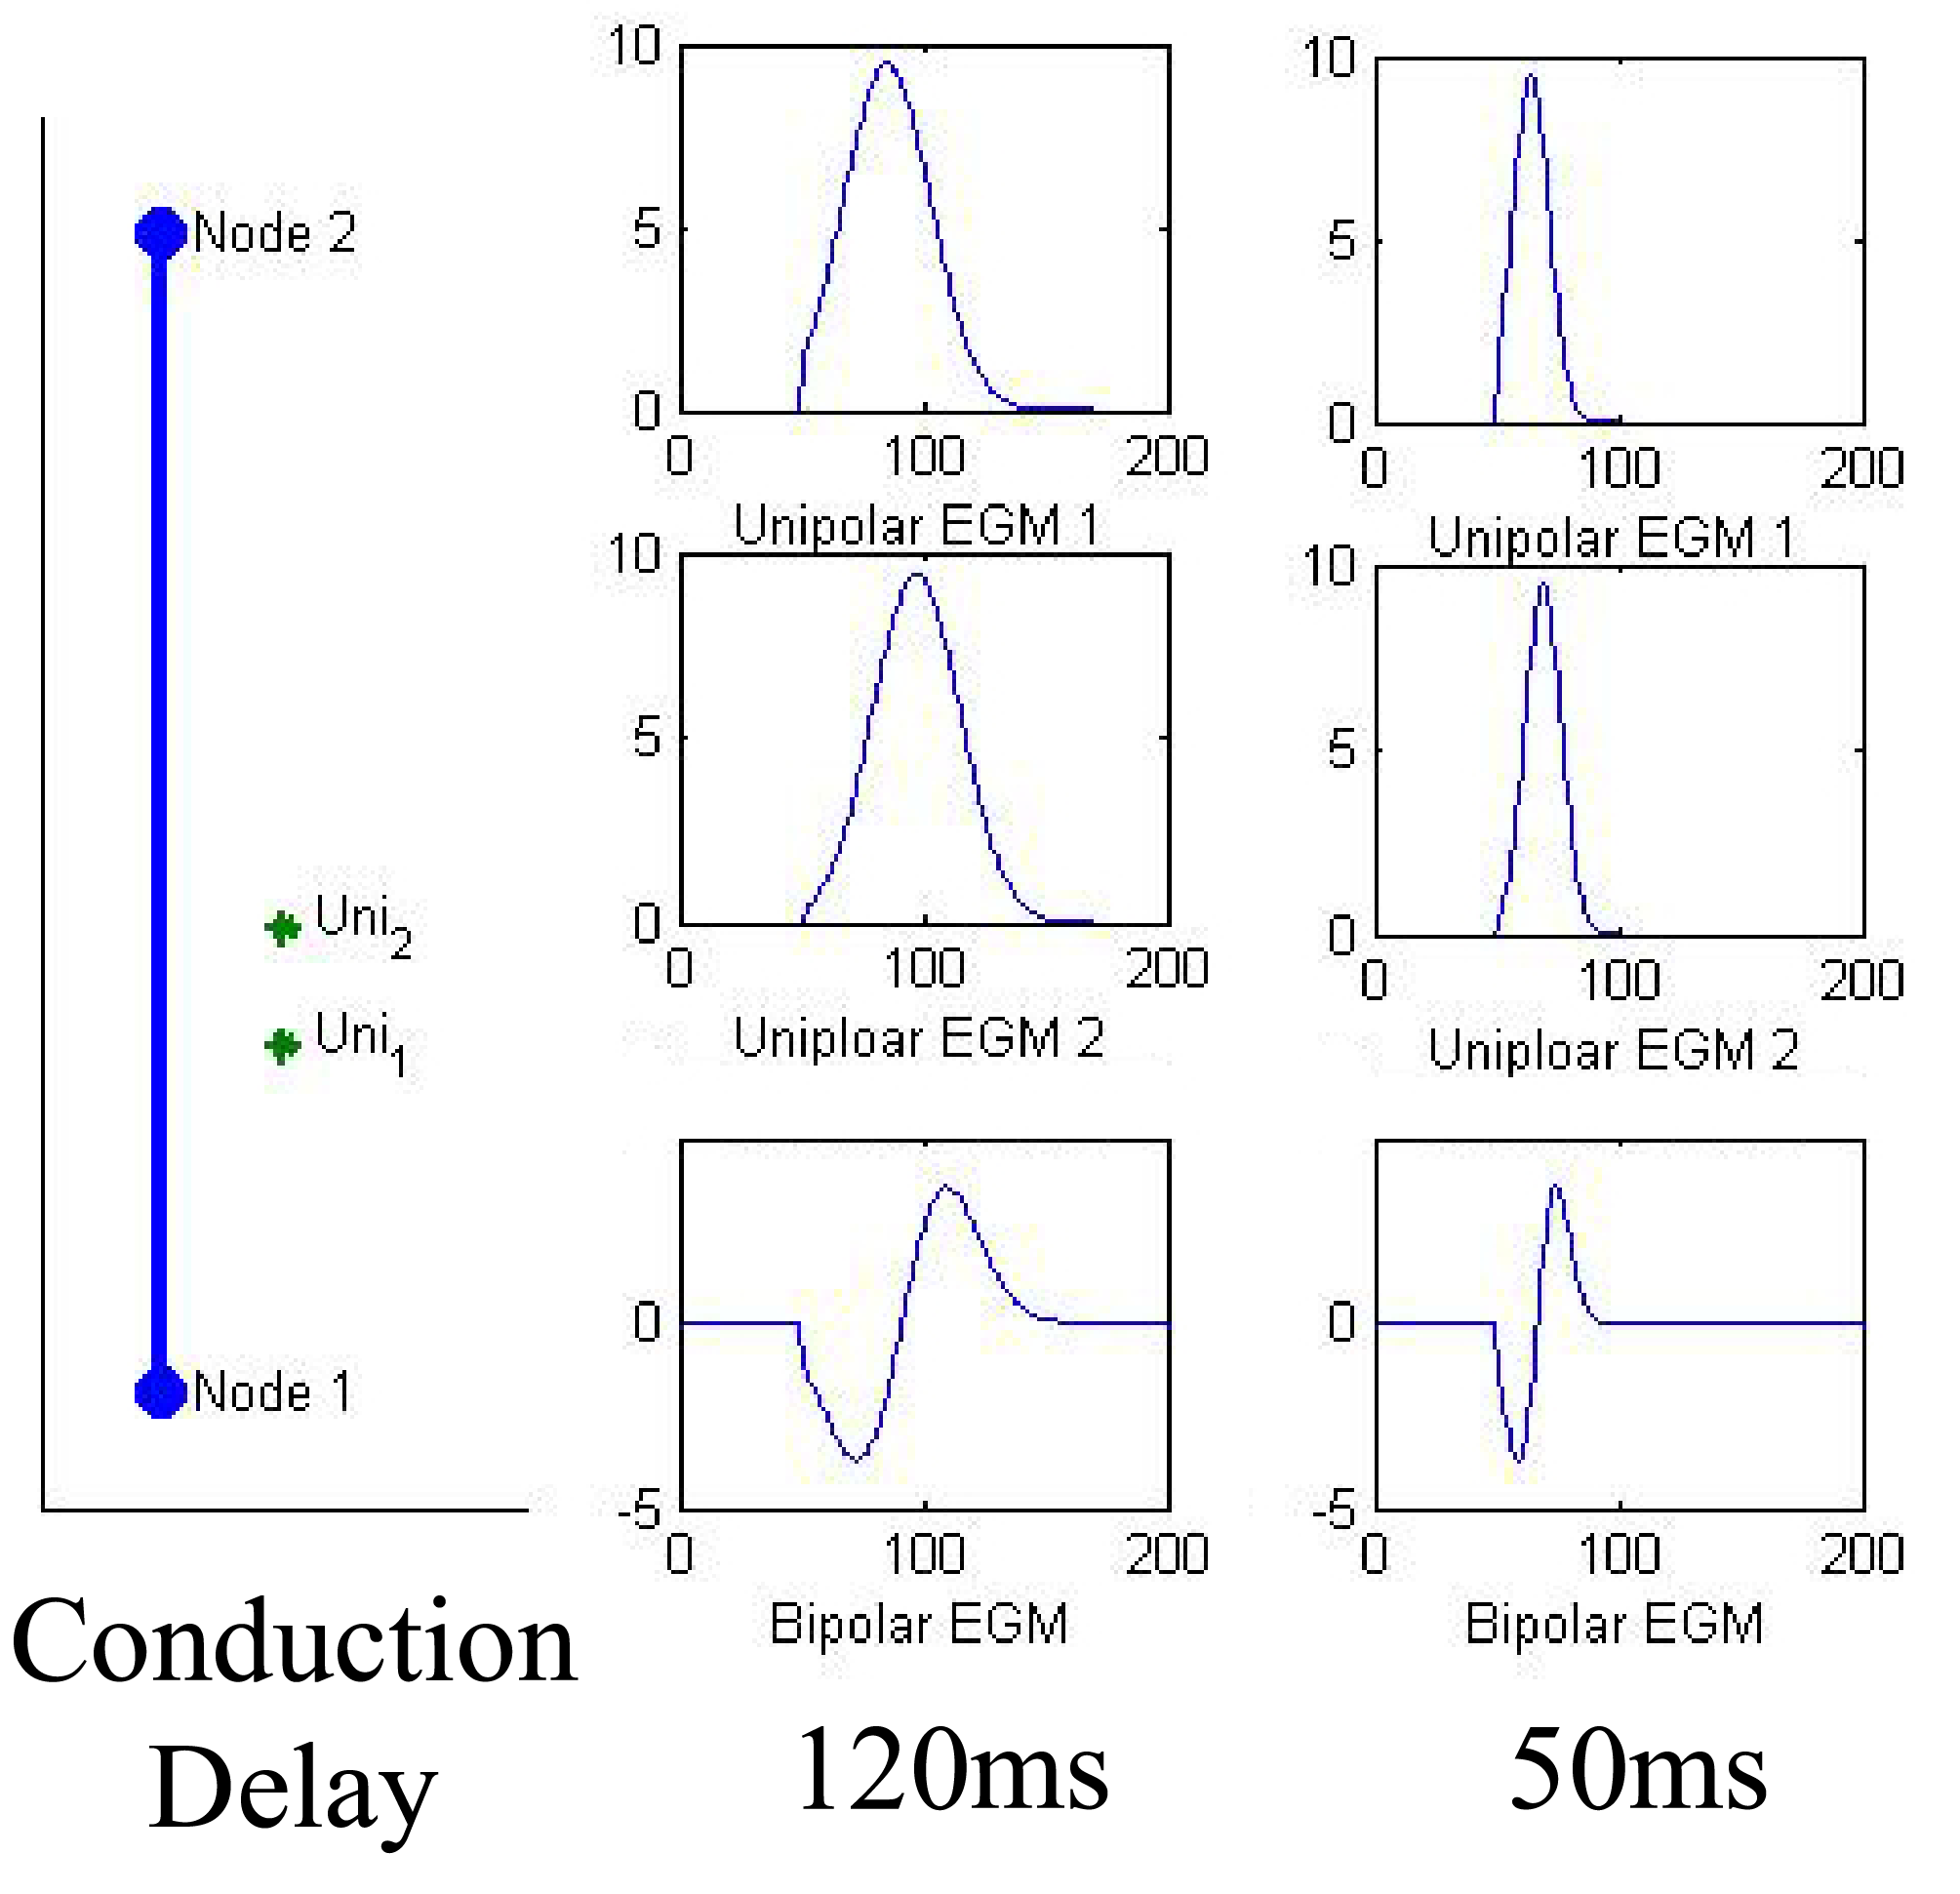
\includegraphics[width=0.7\textwidth]{figs/fig7.png}
%\vspace{-10pt}
\caption{The influence of conduction velocity and probe configuration on the EGM morphology. The left columns show the placement of probes in relation to the path; the right columns show the functional EGM.}
\label{fig:egm_s}
%\vspace{-15pt}
\end{figure}
\section{Interaction with the Heart Model}
In this section, we first introduce a probe model we developed to generate synthetic EGM signals from the EP heart model.
We then use two case study to demonstrate that the probe model enables the EP heart model to evaluate device malfunctions due to sensing errors.
\subsection{Probe Model for Synthetic EGM Generation}
In EP testing and during pacemaker implantation, the local electrical activities, measured as electrogram (EGM) signals, are used to diagnose heart conditions. During heart model construction, we can assign a node automaton at electrode locations and the transitions to the ERP state can be used to represent the local activation events. In a more general setup where electrodes are assigned anywhere within the heart model, a probe model is designed to generate synthetic EGM signals using spatio-temporal information from the proximity to the network of node and path automata. 
According to \cite{recording}, a potential difference is generated when the activation wavefront passes by the electrode. 
The locations of the activation wavefronts are calculated from the locations of the path automata and their current timer values. 
The amplitude of EGM decreases when the activation wavefront moves away from the probe. 
We assume the decrease factor is a function related to the distance between the activation wavefront and the probe. 
The potential difference caused by an activation wavefront to a probe is the signal strength of the path multiplied by the decrease factor. 
The amplitude of EGM from a probe is the sum of potential differences caused by all activation wavefronts. The bipolar EGM is the subtraction between two unipolar EGMs. 
\figref{egm_s} shows that this probe model captures timing properties of EGM and the functional shape of the EGM impulses. The probes can be placed anywhere within the heart model and generate clinically-relevant EGMs. 

\begin{figure}[!t]
\center
%\vspace{-15pt}
		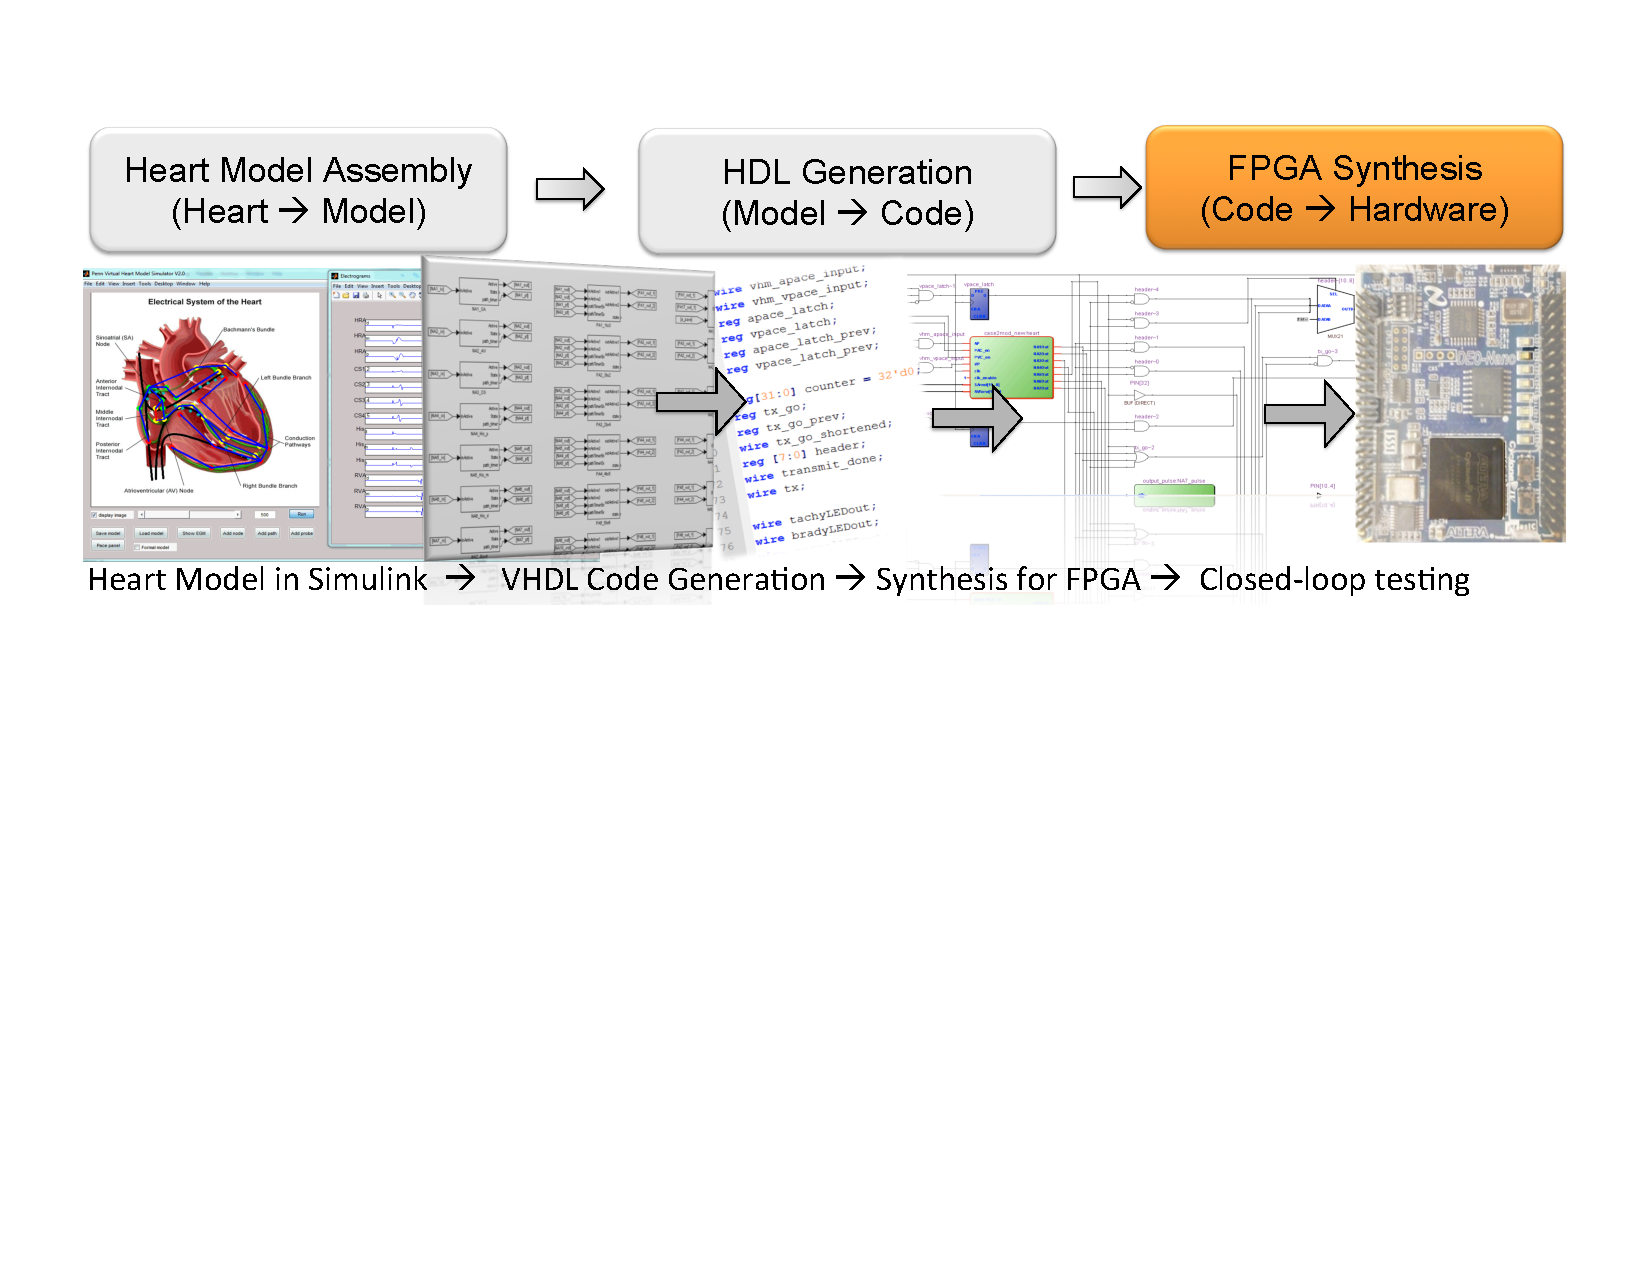
\includegraphics[width=0.98\textwidth]{figs/modeling_heart.pdf}
%\vspace{-10pt}
\caption{The heart model was developed in Matlab/Simulink and code was automatically generated to operate on an FPGA platform for platform-level testing.}
\label{fig:modeling_heart}
%\vspace{-15pt}
\end{figure}

\begin{figure}[t]
\center
\vspace{-10pt}
		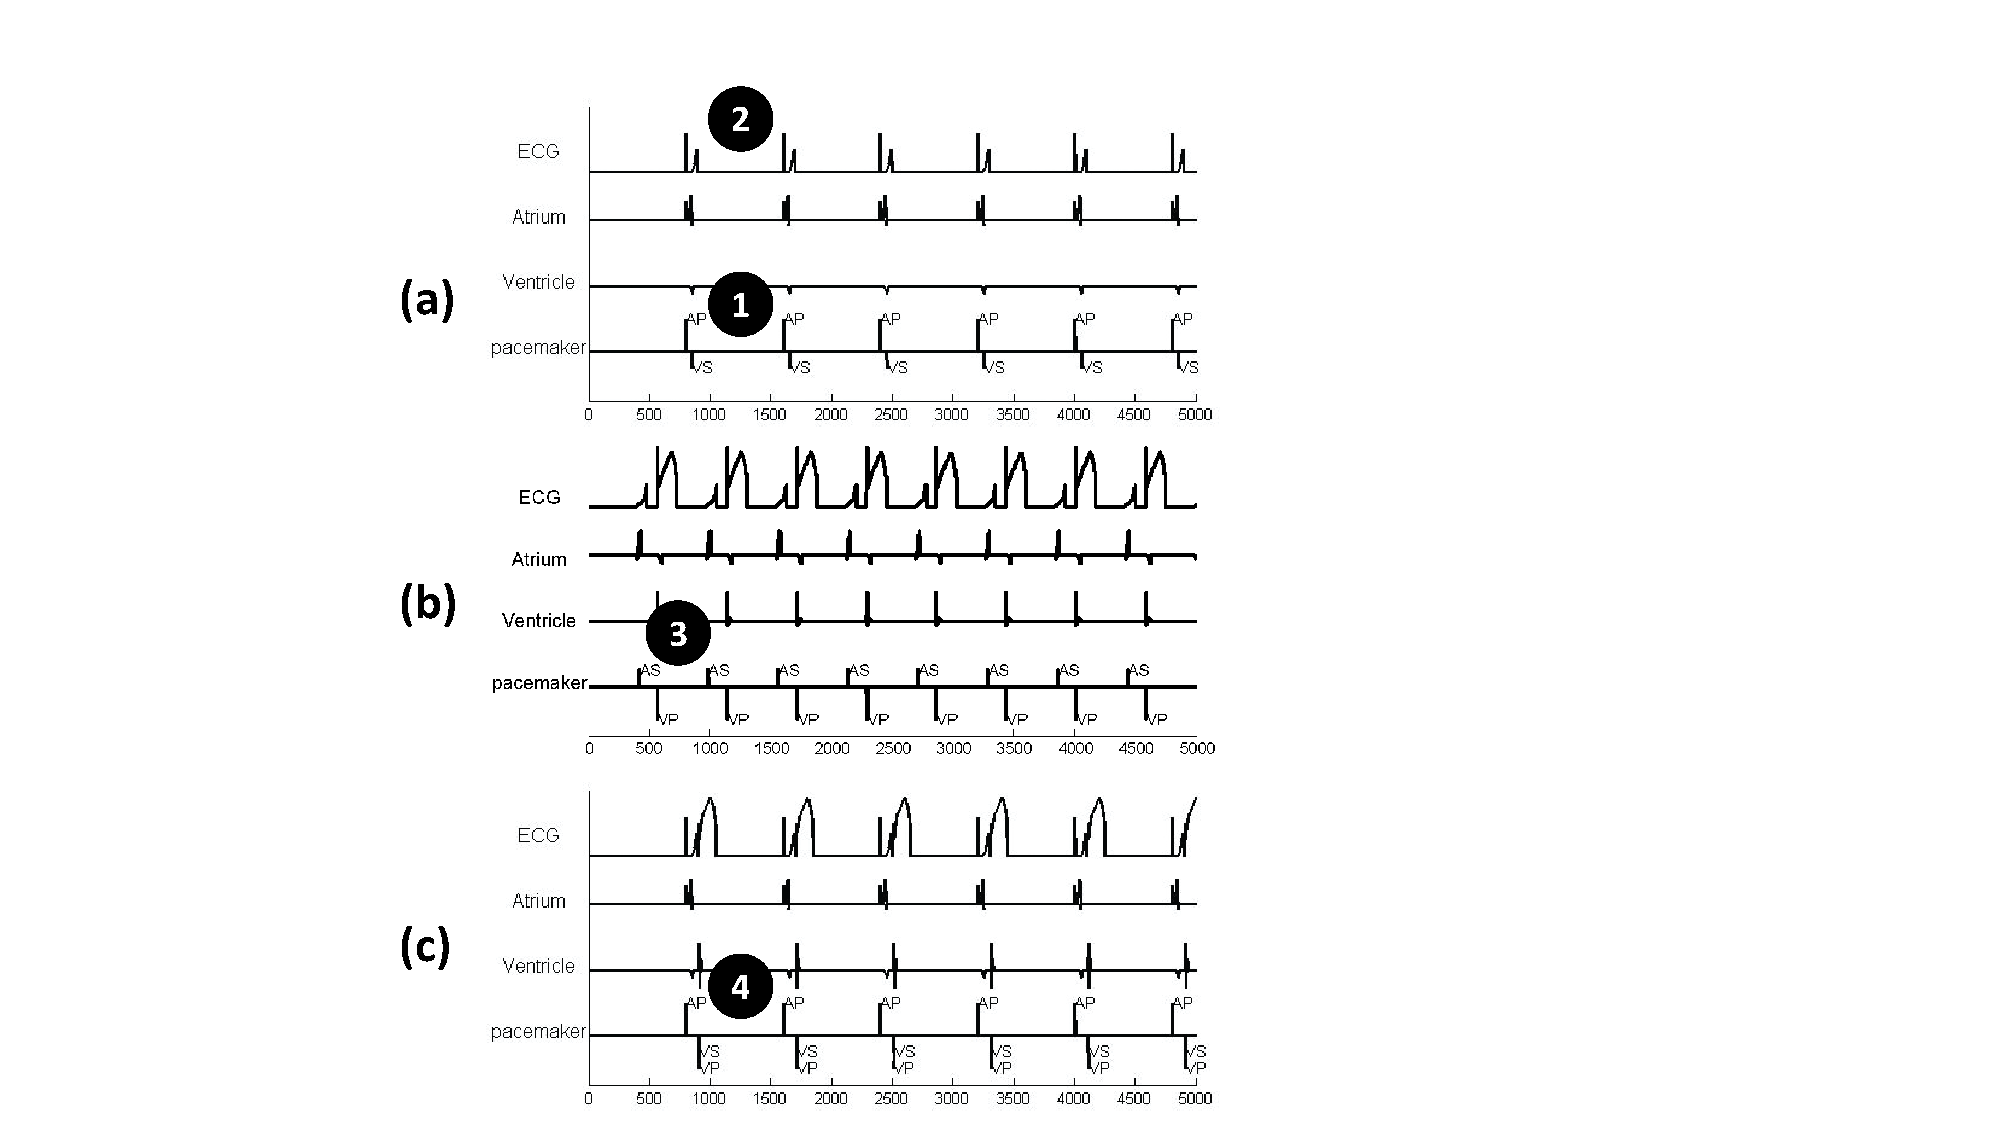
\includegraphics[width=0.6\textwidth]{figs/crosstalk_all.pdf}
%\vspace{-20pt}
\caption{Crosstalk between pacemaker leads with high sensitivity in the ventricle, adjusted sensitivity and ventricular safety pacing}
\label{fig:crosstalk}
%\vspace{-15pt}
\end{figure}
With the sensing model, the heart model structure can be used to identify safety hazards caused by sensing errors.
\subsection{Pacemaker Oversensing and Crosstalk}
Oversensing is a general term for inappropriate sensing caused by noise or far-field signals. It's very common among pacemaker malfunctions and it may result in failure to pace (\cite{med2, leads}), competitive pacing and inappropriate therapy. Crosstalk is a special case for oversensing which occurs when the pacemaker stimulus in one chamber is sensed in the other chamber. It happens when two leads are close to each other or pacing signal in the other chamber is too strong. It is common that the ventricular lead is placed in the right ventricle outflow tract, which is close to the atrium (\cite{icd}). \figref{crosstalk}(a) shows simulated EGMs from a patient with bradycardia and complete heart block. During atrial pacing (AP), the pacing signal is sensed by the ventricular lead 53 ms after the AP. (Marker 1) It is treated as ventricular sense (VS) signal and thus inhibits the subsequent ventricular pacing (VP). This is indicated by no QRS-wave in the ECG channel. (Marker 2) For a patient with complete heart block this will cause dangerous ventricular asystole, meaning a long time without ventricular events.  

Increasing the sensing threshold of the ventricular channel can prevent false sensing. In \figref{crosstalk}(b), the small signals in ventricular EGM are ignored and ventricular pacing are successfully delivered. 


%%%%%%%%%%%%%%%%%%%%%%%%%%%%%%%%%%%%%%%%%%%%%%
\begin{figure}[t]
\centering
\vspace{-10pt}
		%\subfigure [\small]{
		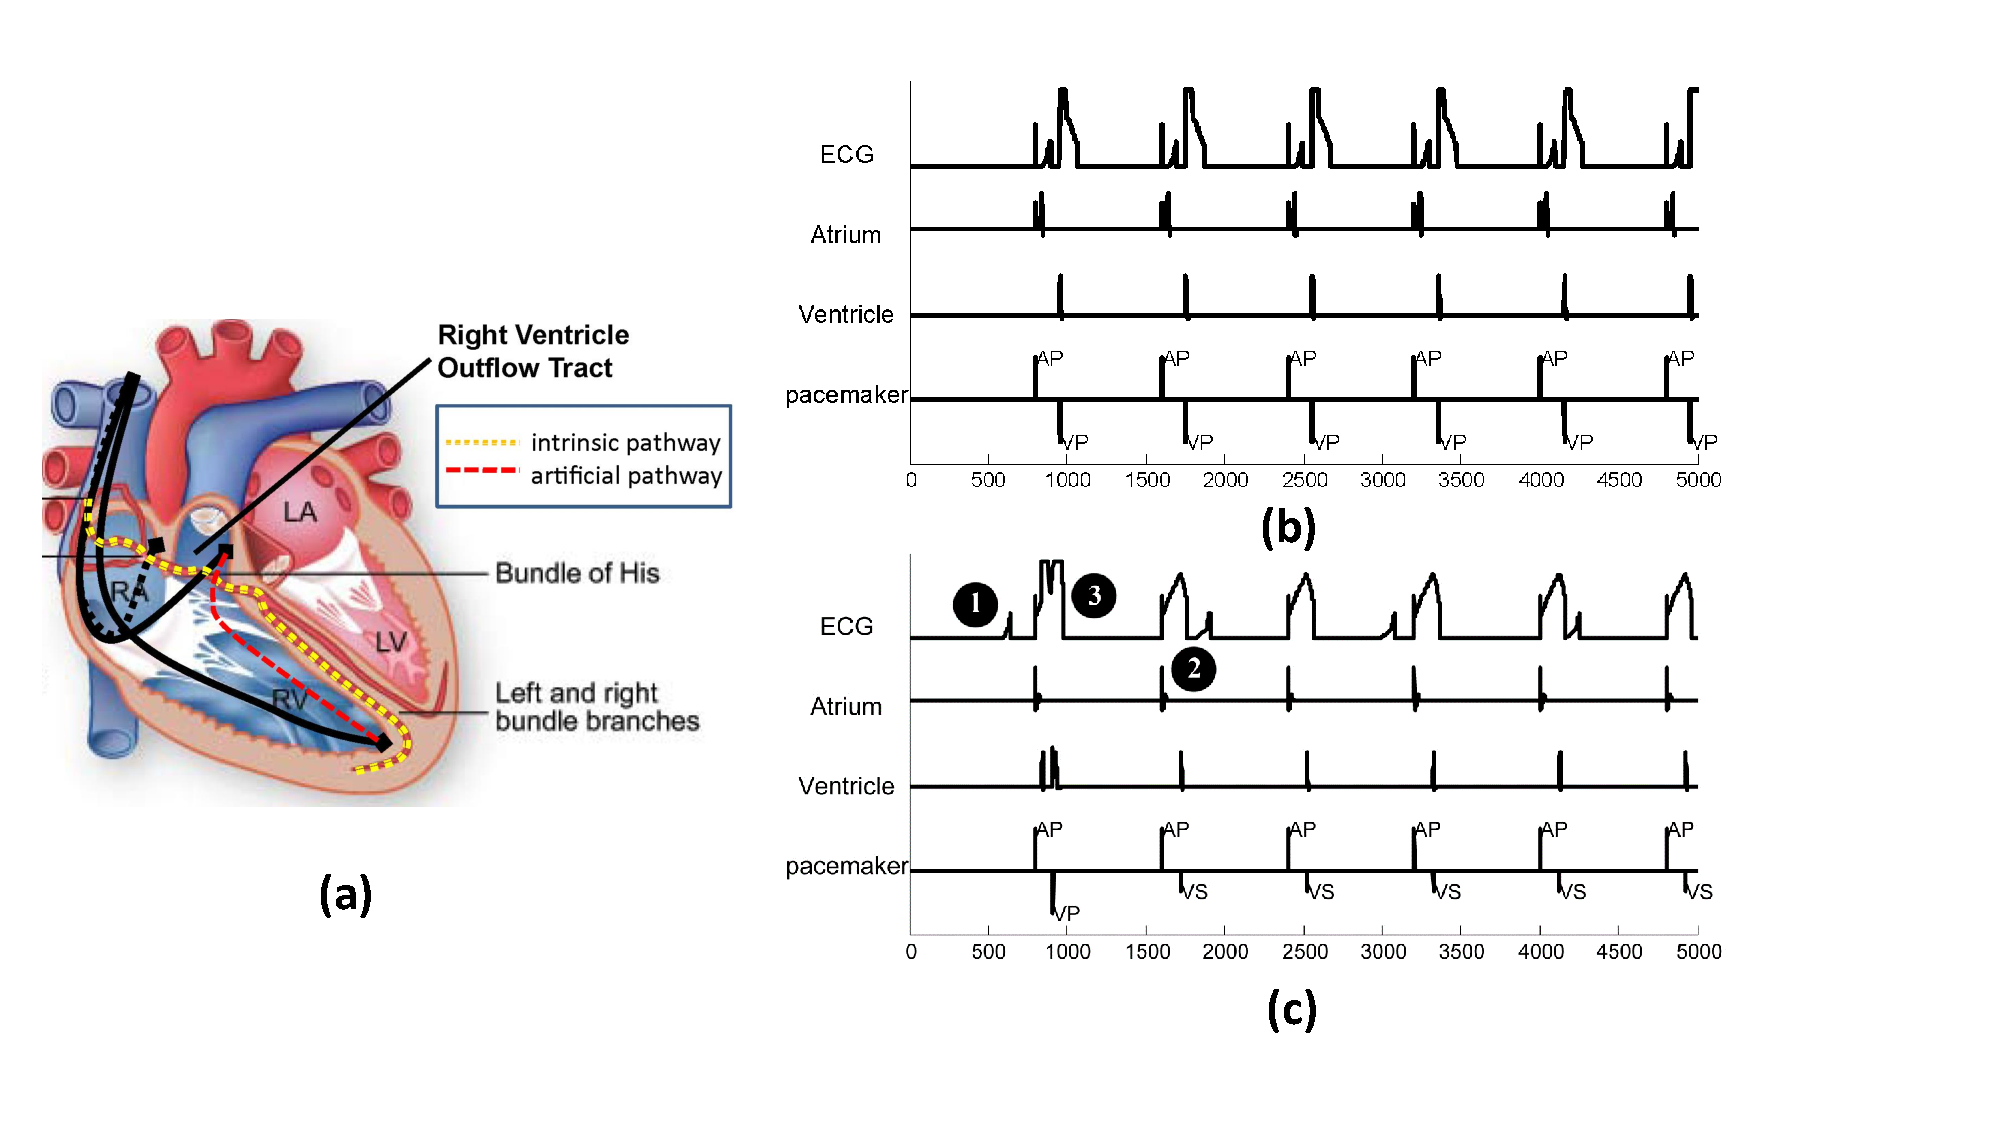
\includegraphics[width=\textwidth]{figs/dislodge_all.pdf}
		%} 
		%\subfigure [\small]{
		%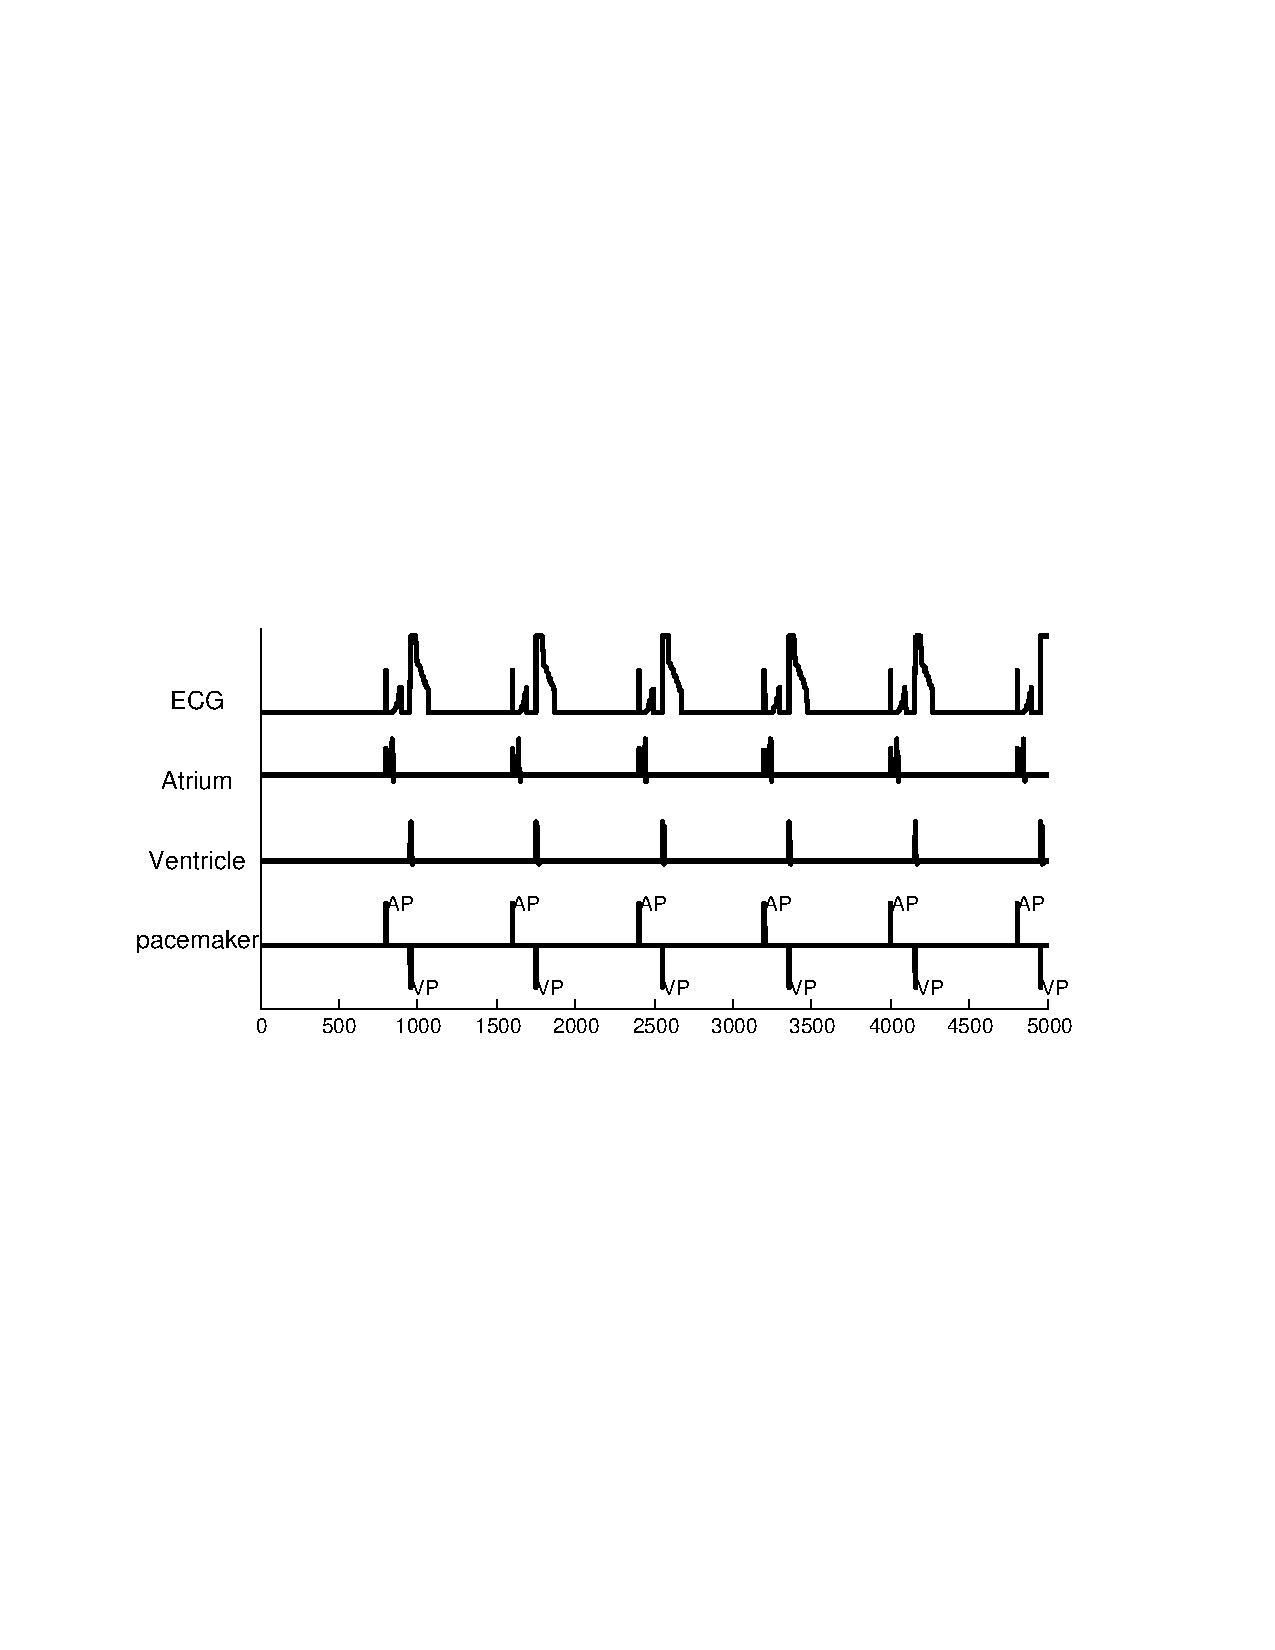
\includegraphics[width=0.36\textwidth]{figs/dislodge_norm.pdf}
		%\label{fig:dislodge_norm}
		%} 
		%\subfigure [\small] 
		%{
		%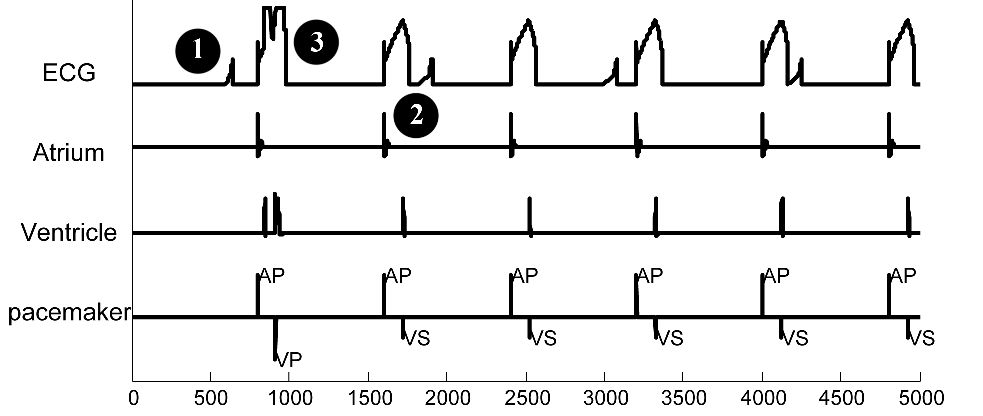
\includegraphics[width=0.36\textwidth]{figs/dislodge_new.pdf}
		%\label{fig:dislodge}
		%} 
%\vspace{-5pt}
\caption{\small (a) Dotted line shows the location where the atrial lead should be (b) Pacemaker function before lead dislodge. (b) Pacemaker function after lead dislodge}
		\label{fig:dislodge_all}

%\vspace{-15pt}
\end{figure} 
%%%%%%%%%%%%%%%%%%%%%%%%%%%%%%%%%%%%%%%%%%%%%%


\subsection{Lead Displacement}
Lead displacement affects many patients and can result in inappropriate or ineffective therapy. \figref{dislodge_all}. (b) shows the simulation result for the pacemaker function when the leads are in their designated location. From the figure we can observe: 1) Each P-wave is initialized by an Atrial Pace signal. 2) Each QRS complex is initiated by a ventricular pacing signal. 3) The interval between AP and VP is 150 ms, which matches the programed AVI period.

%%%%%%%%%%%%%%%%%%%%%%%%%%%%%%%%%%%%%%%%%%%%%%
 %\begin{figure}
%\center
%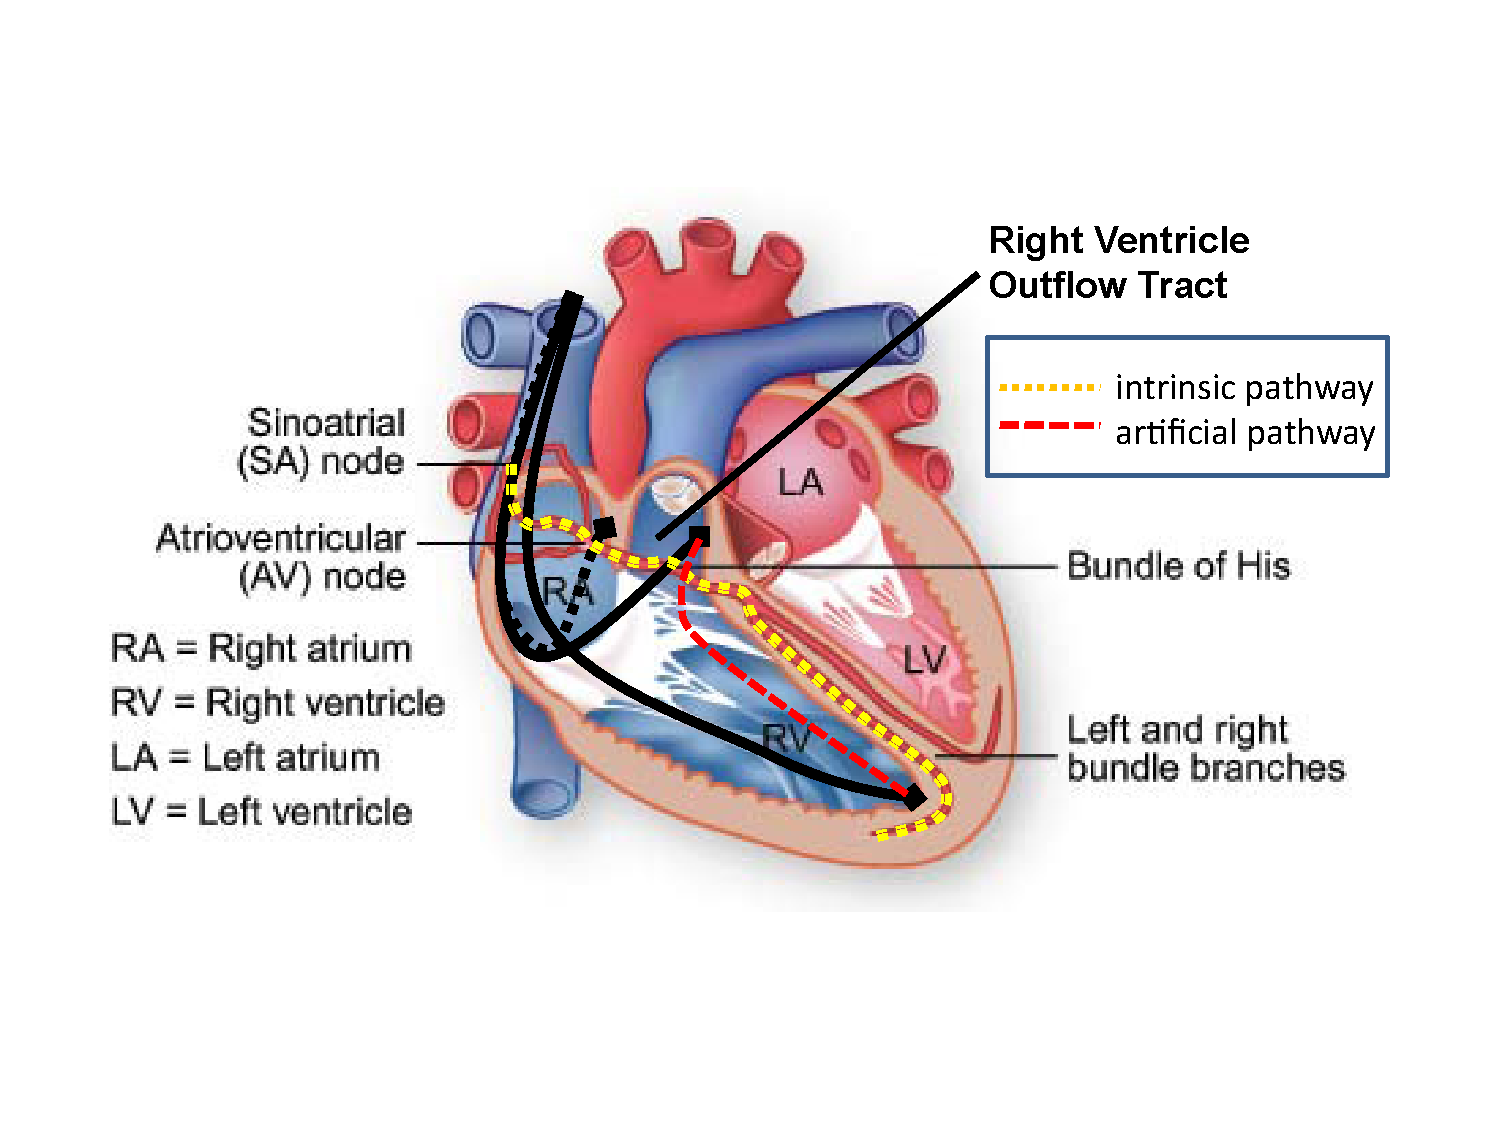
\includegraphics[width=0.7\textwidth]{figs/race_cond.pdf}
%\caption{Dotted line shows the location where the atrial lead should be}
%%\vspace{-15pt}
%\label{fig:race_cond}
%\end{figure}
%%%%%%%%%%%%%%%%%%%%%%%%%%%%%%%%%%%%%%%%%%%%%%

One common case for lead dislodge is shown in \figref{dislodge_all}.(a), where the atrial lead has fallen into the right ventricle outflow tract. In this case the atrial lead senses from the ventricle rather than atrium and atrial pacing will initiate a ventricular event. \figref{dislodge_all}.(c) shows the simulated EGMs in this case. The figure reveals several facts: 1) No P wave is sensed or tracked (Marker 1). 2) Atrial Pace initiates an abnormal, wide QRS which is then sensed by the ventricle lead (Marker 2). 3) Intermittent appearance of VP on QRS 110 ms after the AP. The ventricular lead can receive signal from: 1) pacing signal sent from the atrial lead, 2) the intrinsic A-V conduction path. The two paths are shown in \figref{dislodge_all}.(a) and form a timing race condition. When the signal from the atrial lead arrives the ventricular lead first, it will trigger VS. If the intrinsic signal arrives the ventricular lead during the VSP sensing window (defined in previous section), it will trigger VSP. Although the pacing is 'safe' because the pacing is early enough to avoid the vulnerable refractory period, the damage caused by pacing on depolarized tissue is currently a matter of much investigation.\\



\section{Heart-on-a-Chip Platform}
Platform testing remains the primary means to verify and validate device software. Currently testing is performed by feeding recorded open-loop heart signals to the device and evaluating the device output. Consequently, the change in the state of the heart condition, in response to device output, is not taken into account. Thus, device malfunctions involving state changes due to multiple closed-loop interactions will not be captured during open-loop testing. 

To this effect, the heart model described above is also implemented on hardware platform (\figref{modeling_heart}) for closed-loop testing. Since each heart model is a network of node and path automata running concurrently, we implemented the heart model on an FPGA, so that increasing in the number of nodes and paths would not affect real-time constraints. The second generation heart model implementation has been implemented on a lower cost fast micro-controller platform. The fast clock ensures that executions of all nodes and paths can be finished within 1ms. The Heart-on-a-Chip platform includes a heart model implementation which is able to represent common heart conditions such as bradycardia, tachycardia, heart block, etc (for mode details refer to \cite{VHM_proc}). The parameters of the heart model can be changed at run-time by either switching among pre-defined parameter sets, or sending values directly to the model through a user interface in Matlab. A monitoring system observes logical interactions between heart model and the pacemaker and checks them against safety invariants at run-time. 

As shown in (\figref{HOC}), with an analog interface the heart model can interact with a commercial pacemaker in real time. Our analog interface uses an optical isolation circuit to separate the pacemaker circuit and the heart implementation. Signals generated from the heart are attenuated to the appropriate level to interact with a Boston Scientific pacemaker and analog pacing signals are converted to pacing events received by the heart model. 

\begin{figure}[!b]
\center
%\vspace{-15pt}
		\includegraphics[width=0.8\textwidth]{figs/PVS.pdf}
%\vspace{-10pt}
\caption{Heart-on-a-Chip testbed for real-time closed-loop testing of the pacemaker or model of the pacemaker with the heart model on the hardware platform}
\label{fig:HOC}
%\vspace{-15pt}
\end{figure}

% \subsubsection{Abstracting Beat-to-beat Dynamics}
% \subsubsection{Abstracting Conduction Delays with Path}
% \subsubsection{Merging Activation-generating Nodes}
% \subsubsection{Replace ERP Blocking With Non-deterministic Conduction}
% \subsubsection{Replace }




